\part{Analysis of sorting}  
\label{ch:effsort}

\chapter{The problem of sorting, selection sort} %--------------------------------------------
\label{sec:sortingproblem}
Sorting (especially integers or words) is ubiquitous in computing.
Sorting also makes many other problems easier, e.g., selection and finding duplicates.
The problem of sorting is as follows. 

\begin{Definition}
Given $n$ \defnfont{keys} $a_1, \dots , a_n$ from a totally ordered set, put them in increasing order. 
The keys may be just part of a larger data record.
\end{Definition}
\begin{Boxample}[3]
Sort the integers $\set{42, 7, 911, -2}$ with $\leq$ 
and the words $\{$\textit{banana, computer, Auckland, bamboo}$\}$ with  alphabetical (lexicographic) order.
\end{Boxample}



\section{Properties of sorting algorithms}
\begin{Definition}
A sorting algorithm is \defnfont{comparison-based} if it only uses the order relation to compare keys.
\end{Definition}

This is consistent with the ADT (Abstract Data Type), object-oriented approach. 
There are other algorithms like bucket sort, radix sort, etc. that do not do this. 
They use properties of the data representation such as the decimal expansion of keys.
We only analyse comparison-based algorithms, since they work for general data. Note that the data structure used for sorting is important. 
Sorting an array is a different problem from sorting a linked list. 
However, these differences affect  only efficiency, not correctness, and for correctness we can (and should) consider the algorithm as acting on a general list. 


We consider only two elementary operations: a \boldfont{comparison} of two items and a \boldfont{move} of an item.
For a comparison, we choose keys $x$ and $y$ and answer the question ``is $x<y$?" (or maybe we ask which of $x < y, x = y, y < x$ is true). 
There are two main types of move-related operations. 
\begin{itemize}
\item We can \boldfont{swap} the position of elements (at positions $i$ and $j$ say). 
Each swap requires 3 updates of variables.
\item Another way is to insert the element in the list at position $i$ after position $j$ and remove it from its current position.
\end{itemize}

If the list is implemented using an array, then insertion-deletion is expensive ($\Theta(n-j)$ data moves in worst case), 
since elements must be moved along, and hence this is not an elementary operation. Then swaps are better.

If the list is implemented as a linked list, then insertion is cheap ($\Theta(1)$ data moves in worst case).
So we usually do that instead of swapping.

\begin{Definition}
A sorting algorithm is \defnfont{in-place} if it only uses fixed additional space, independent of $n$.
It is \defnfont{stable} if records with equal keys have their order unchanged by the algorithm.
\end{Definition}

% \begin{Boxample}
% A stable sorting of the array of pairs $[(2, a), (1, b), (3, b), (1, a)]$ based on their integers is
% $[(1, b), (1, a), (2, a), (3, b)]$ and based on their characters is $[(2, a), (1, a), (1, b), (3, b)]$.
% \end{Boxample}


\section{Selection sort} %----------------------------------------------------
\label{sec:selectionsort}
The sorting algorithm \defnfont{selection sort} works as follows.
We think of the list as an unsorted part followed by a sorted part.
The list starts completely unsorted, and we extend the sorted part until the list is completely sorted.
We grow the sorted part in the following way.
\begin{itemize} 
  \item Find the maximum element of the unsorted part of the list by sequential
  scan, and move it to the end of the sorted part. Iterate.
\end{itemize} 

This is perhaps the most obvious sorting algorithm. 
It makes the smallest possible number of swaps of any comparison-based sorting algorithm, 
so may be useful if data moves are VERY expensive.
Is it clearly inefficient, since useful comparison information gathered in each pass is forgotten.

\begin{algorithm}[H]
  \caption{Selection sort.}
    \label{alg:selsort}
\begin{algorithmic}[1]
\Function{Selsort}{list $a[0..n-1]$}
%\State $n \gets \texttt{a.size()}$ 
\For{$i \gets n-1$ \text{to} $0$} 
	\State $k \gets $ \texttt{findmax}($a[0..i]$) \Comment{$i$ is the last unsorted position}
	\If{$k \neq i$} 
		\State \texttt{swap}($a,i,k$)
	\EndIf
\EndFor
\State \Return{$a$}
\EndFunction
\end{algorithmic}
\end{algorithm}

\begin{Boxample}[0]
Complete the following selection sort process.
\begin{center}
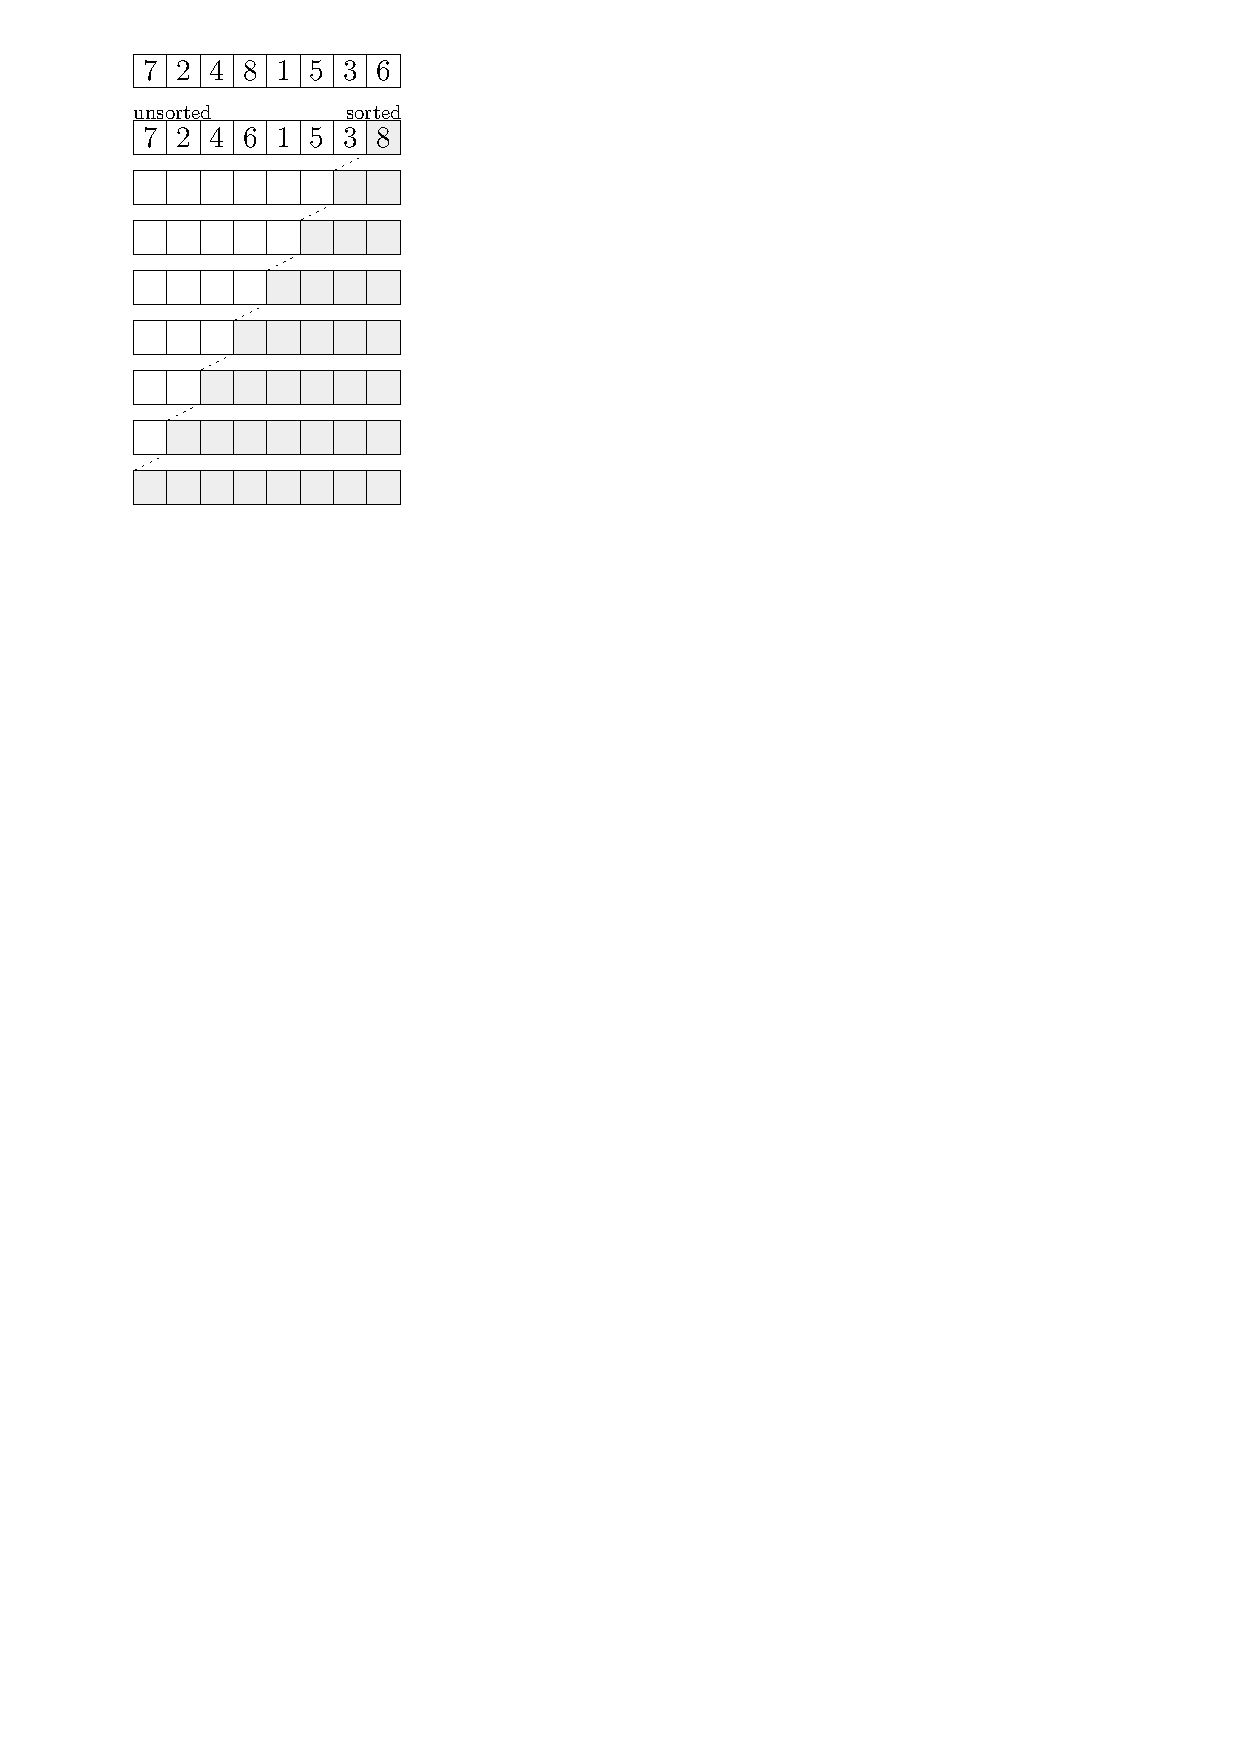
\includegraphics{SelectionSort}
\end{center}
\end{Boxample}

We now analyse the properties of selection sort.

\section{What is the running time?}
Finding the maximum of $a[0..i]$ by sequential search takes $i$ comparisons,
so the total number of key comparisons is $\sum_{i=0}^{n-1} i  = \frac{n(n - 1)}{2}$.
The number of index comparisons is $n$ and the number of swaps is at most $n - 1$.
Hence, the running time is in $\Theta(n^2)$ if we take comparisons and swaps as elementary operations.

\section{Which inputs give the best and worst case?}
The algorithm is very insensitive to the input. 
Its best and worst case running time are very similar. 
The best case is when the list is already sorted; the worst is when every swap is needed, 
and this occurs when the input permutation has no fixed point. 
However the number of comparisons, which usually dominates the running time, is the same for every input.

\section{Is selection sort in-place?}
Yes, selection sort is an in-place sorting algorithm. Convince yourself why.

\section{Is selection sort stable?}
No, selection sort is not a stable sorting algorithm.
\begin{Boxample}[0]
Execute selection sort on the following input to convince yourself that the algorithm is not stable.
\begin{center}
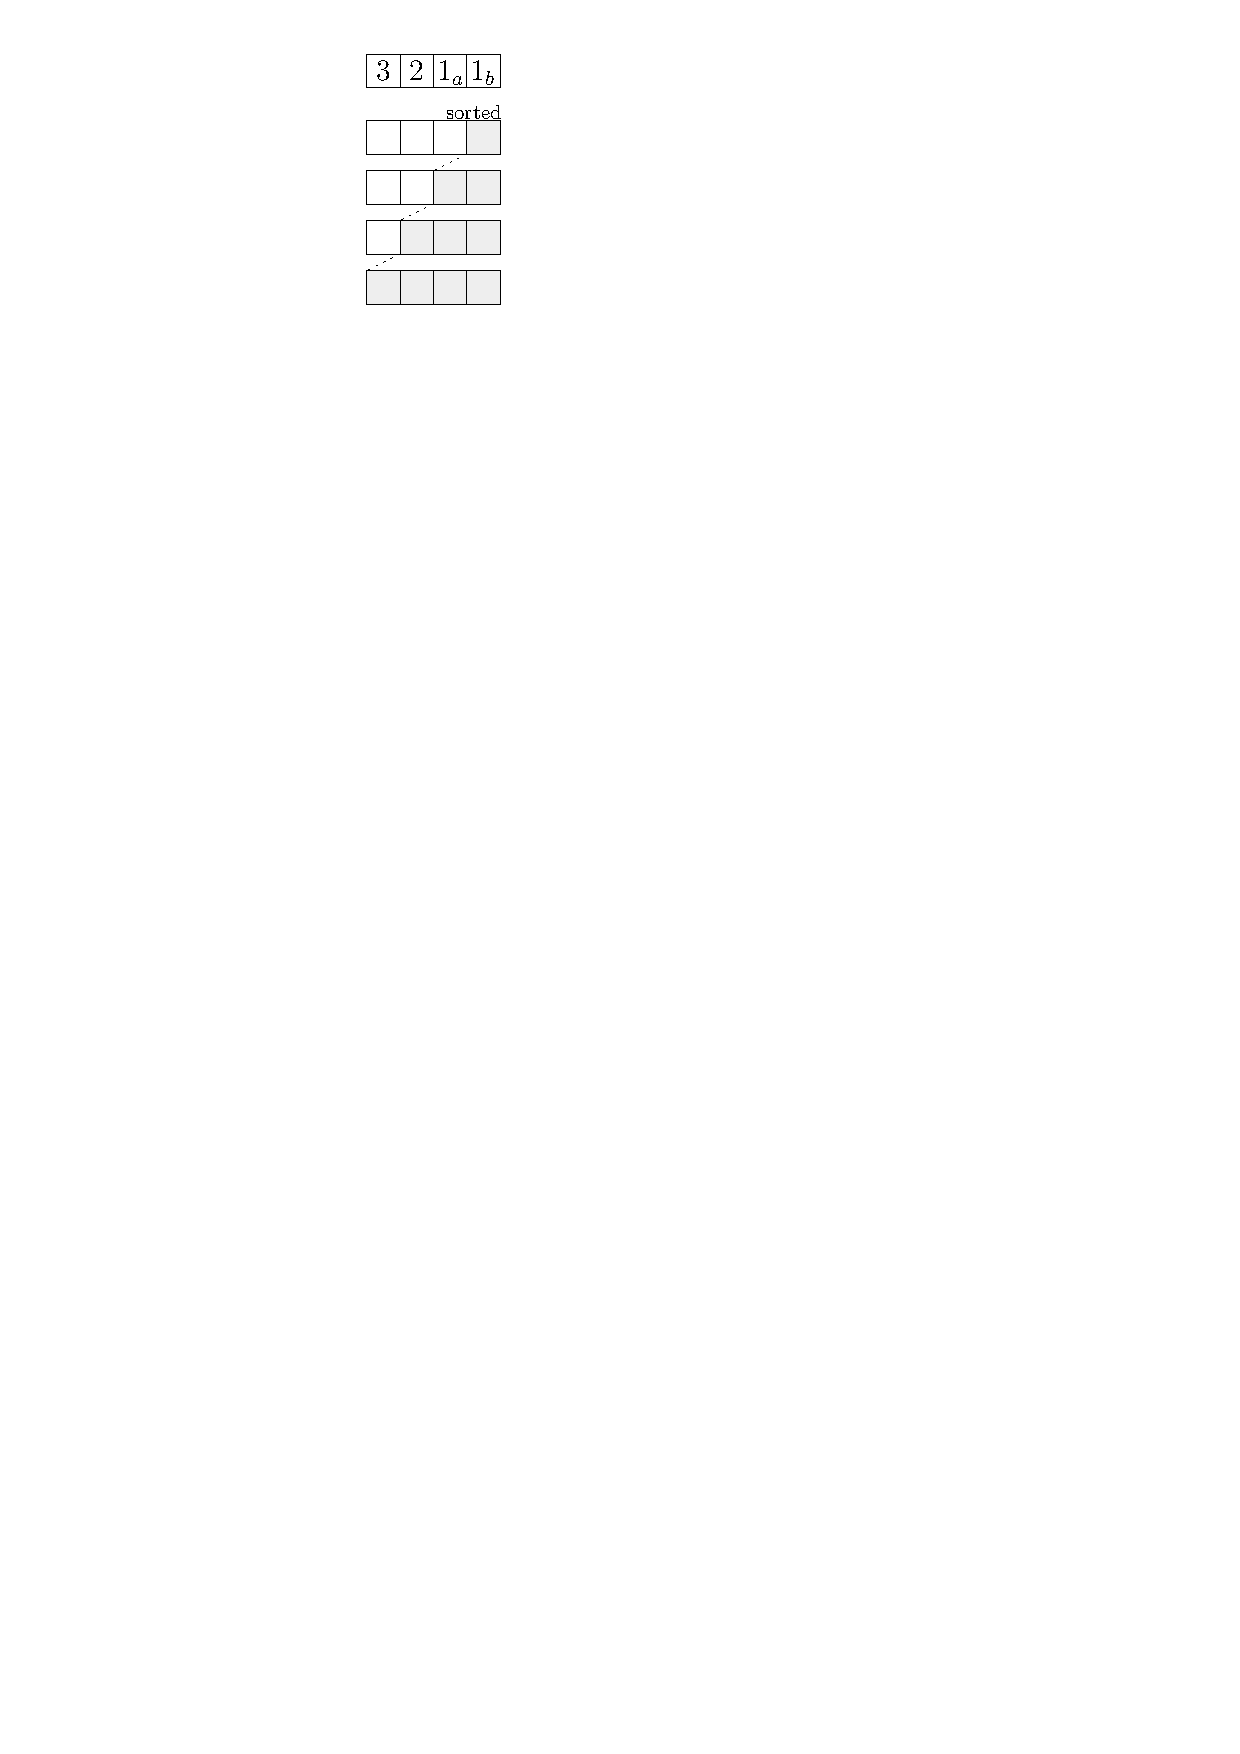
\includegraphics{SelectionSortStable} 
\end{center}
\end{Boxample}

\section{What happens if we run selection sort on a linked list?}
Running time on a linked list is not much different from performance on an array. 
The differences involve swap versus insertion, but comparisons dominate the running time anyway.

Lastly, note that there is no better way to find the maximum using a list than what we have done above. 
But if we change the data structure \dots (see \cref{sec:heapsort} on heapsort).


\chapter{Insertion sort} %----------------------------------------------------
\label{sec:insertionsort}
Similarly to selection sort, in the \defnfont{insertion sort} sorting algorithm we have a sorted part followed by an unsorted part.
We grow the sorted part in the following way.
\begin{itemize}
	\item For each element $x$ in the unsorted part of the input list, 
	scan backward while the preceding element exceeds it. 
	Move $x$ to its correct position. Iterate.
\end{itemize}
This is the sorting method used by card players to arrange cards in a hand.
It works well on small lists, or lists that are nearly sorted.

\begin{algorithm}[H]
  \caption{Insertion sort.}
    \label{alg:insort2}
\begin{algorithmic}[1]
\Function{Insort}{list $a[0..n-1]$}
	%\State $n \gets \texttt{a.size()}$  
	\For{$i\gets 1$ \text{to} $n-1$}  \Comment{$i$ is the first unsorted position}
		\State $j \gets i$  \Comment{$j$ is the element being moved}
		\While{$a[j-1] > a[j]$ and $j > 0$}
			\State \Comment{swap backward to move to right place}
			\State \texttt{swap}$(a,j-1,j)$
			\State $j \gets j - 1$
			%\State $j \gets $ \texttt{findlastinv}($a[0..i]$)
			%\If{a[j]>a[i]}
			%\State \texttt{swap}($a,i,j$) 
			%\EndIf
		\EndWhile
		%\State $a[j+1] \gets a[i]$ \Comment{insert $a[i]$ in correct position}
	\EndFor
	%\If{$j \neq i$} 
	%\State \texttt{swap}($a,i,j$)
	%\EndIf
	\State \Return{$a$}
\EndFunction  
\end{algorithmic}
\end{algorithm}

\begin{Boxample}[0]
Complete the following insertion sort process.
\begin{center}
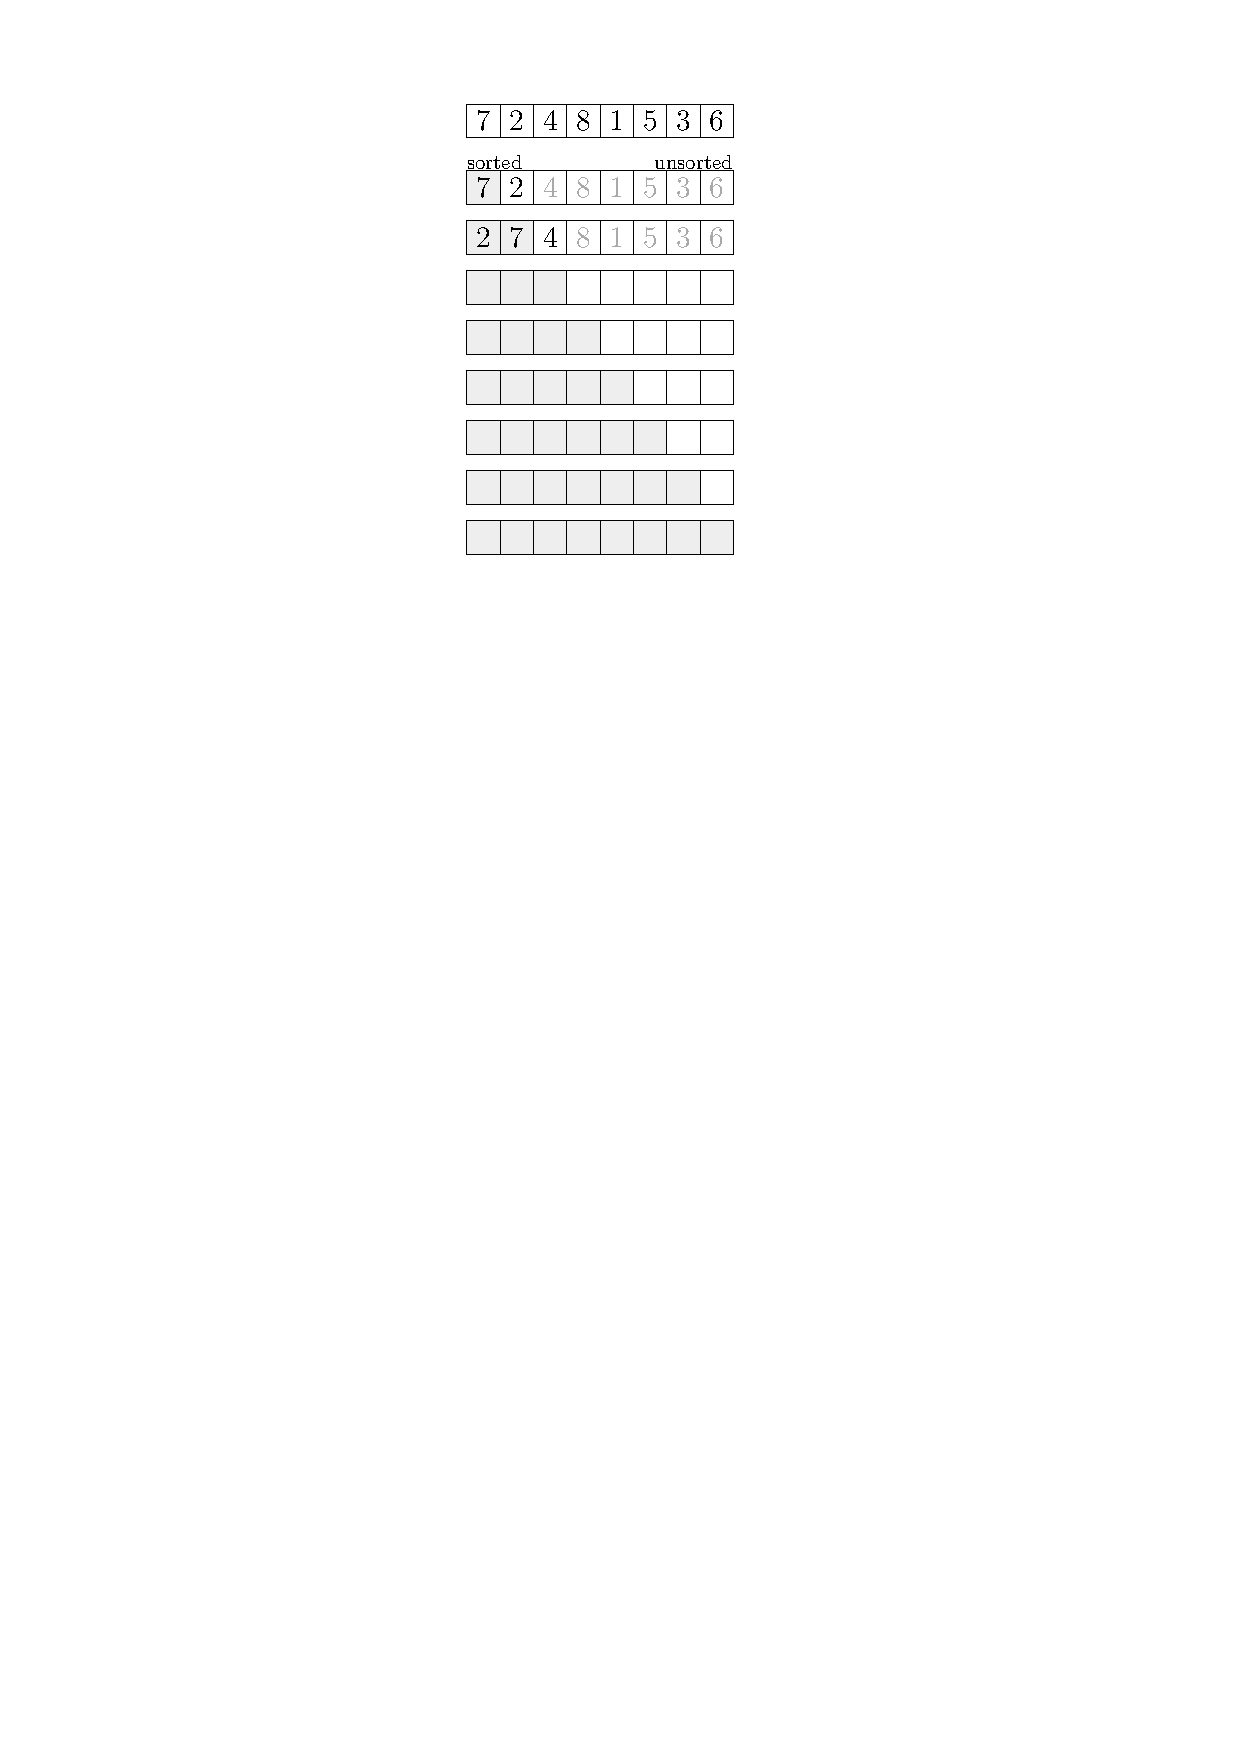
\includegraphics{InsertionSort}
\end{center}
\end{Boxample}


\section{Insertion sort analysis}
The number of key comparisons for fixed $i$ is one more than the number of $j$ such that $j < i$ and $a[i] < a[j]$.
Thus the total number of comparisons is $n-1$ plus the number of \defnfont{inversions}, 
namely pairs $(i, j)$ of indices with $j < i$ and $a[j] > a[i]$ (``out of order" pairs of elements).
This is also thee number of swaps.
In the best case insertion sort runs in linear time.
In the worst case the number of inversions is $n(n-1)/2$ 
(where input is in reverse sorted order) so it runs in quadratic time $\Theta(n^2)$.

\begin{Boxample}[4]
How many inversions are in the permutation $72481536$?
\end{Boxample}

\section{What is the average-case performance of insertion sort on random data?}

\begin{Boxample}[6]
What is the average number of inversions in a random permutation of $\{1,\dots, n\}$?
\end{Boxample}
% \textit{Proof.} For every pair $(i,j)$ with $i\neq j$,  and every permutation $\pi$, 
% this pair is an inversion in exactly one of $\pi$ or the reverse of $\pi$.

\section{Which inputs give the best and worst case?}
Unlike selection sort, insertion sort has running time that is very sensitive to the input. 
As mentioned above, the best case occurs when the input is already sorted, and the worst when the input is in reverse sorted order.

\section{Is insertion sort in-place?}
Yes, insertion sort is an in-place sorting algorithm. Convince yourself why.

\section{Is insertion sort stable?}
Yes.

\begin{Boxample}[0]
Execute insertion sort on the following input to convince yourself that the algorithm is stable.
\begin{center}
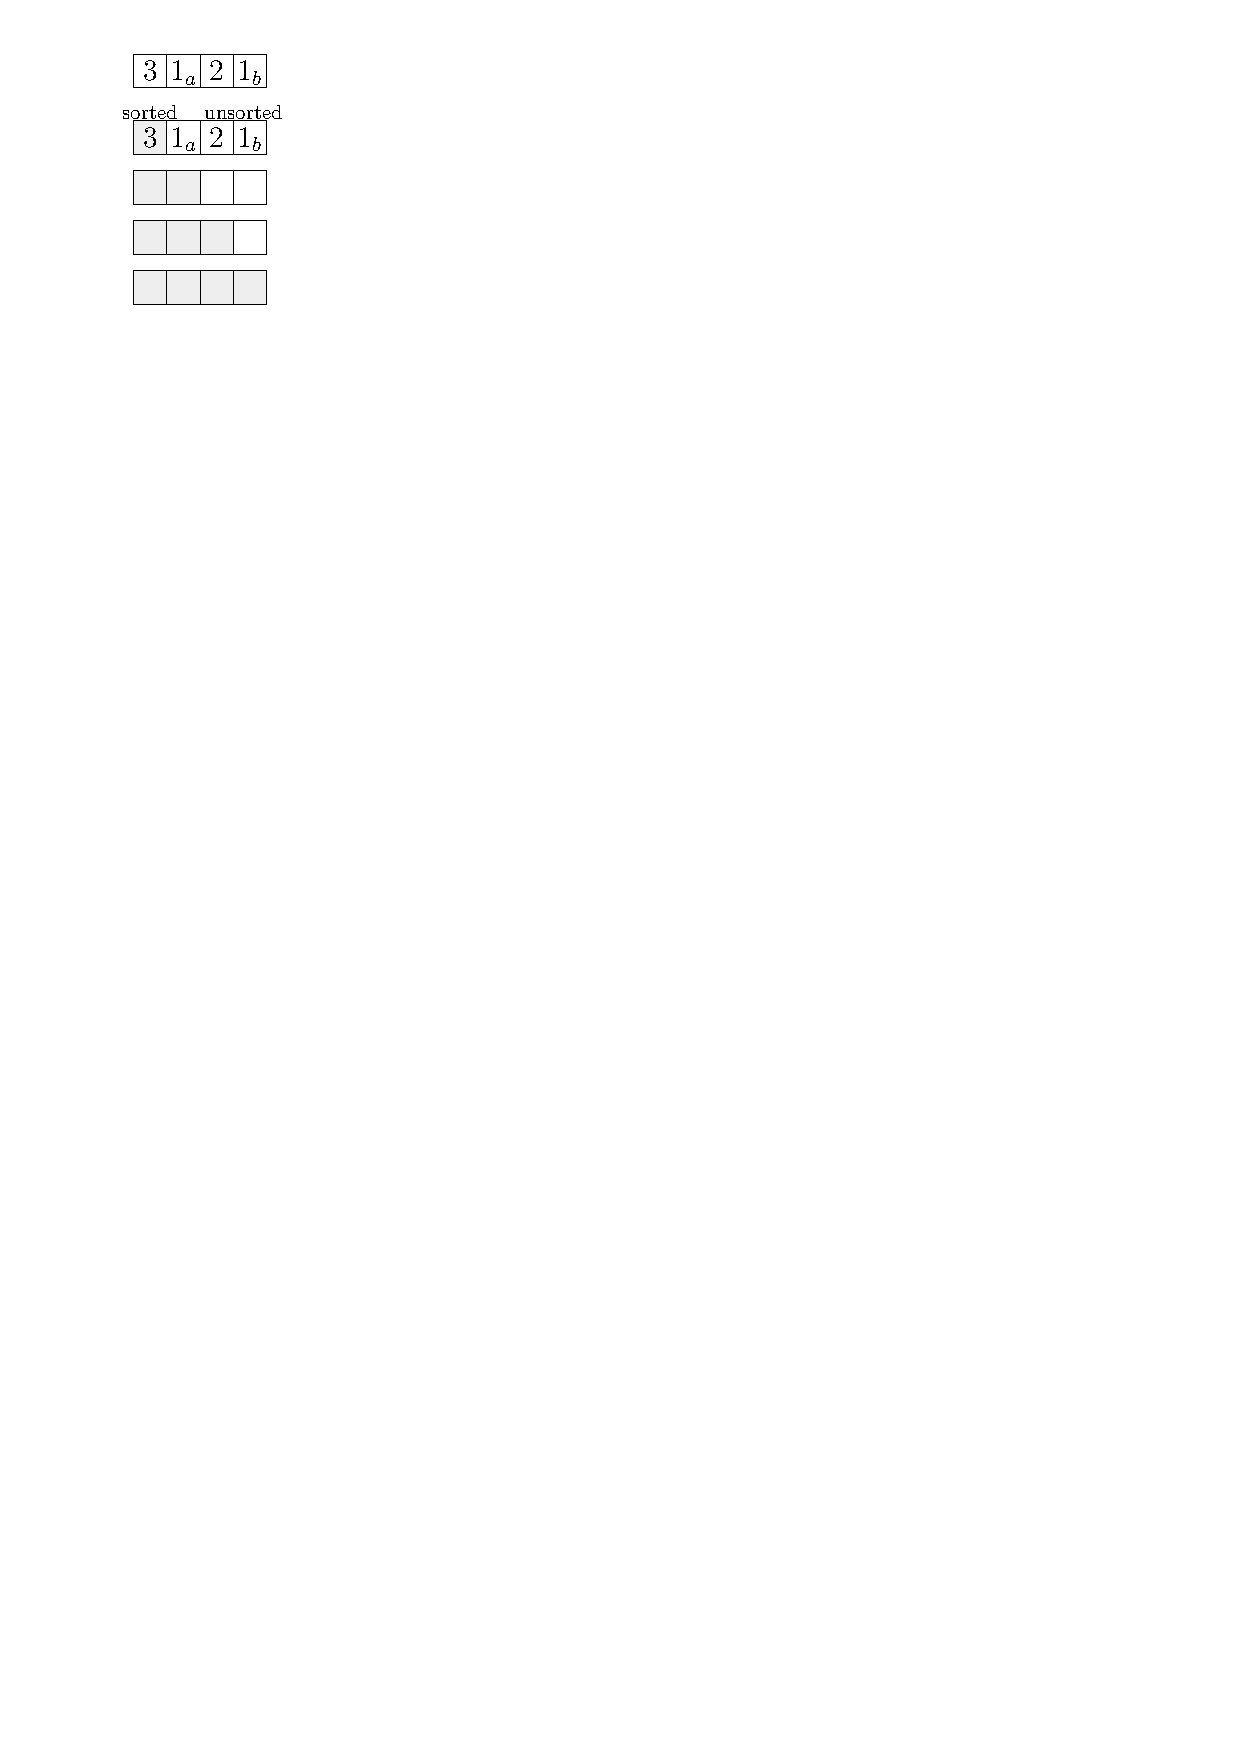
\includegraphics{InsertionSortStable} 
\end{center}
\end{Boxample}

\section{Analysis when implemented on a linked list}
We can reduce the number of data moves if we use a linked list to implement 
the list ADT.
Instead of repeatedly swapping an element, we can remove it from the list and insert it back in the right position.
However, searching to find the right insertion point still takes time in
$\Theta(n^2)$ in the worst case.

\section{How can we improve insertion sort?}
On an array, we can reduce the number of comparisons by using binary search (see future lecture) to find 
the insertion point. However, the swaps still take time in $\Theta(n^2)$ as above, so this is of little use.

We can improve by changing the algorithm somewhat.
We can move elements to the left using big steps, gradually reducing the 
step size to 1. This is called \defnfont{Shellsort} (D. Shell, 1959). 
\begin{itemize}
  \item Fix $h = n/2$. Run insertion sort on the sublists formed by taking 
every $h$th element. Iterate, reducing $h$ to $1$ systematically. 
\end{itemize}
The key property is that each run removes inversions and none are 
restored by later runs. The last run is just insertion sort, but on a file that 
is almost sorted.

\begin{Boxample}
An example of Shellsort with $h = 5, 3, 1$.
\begin{center}
  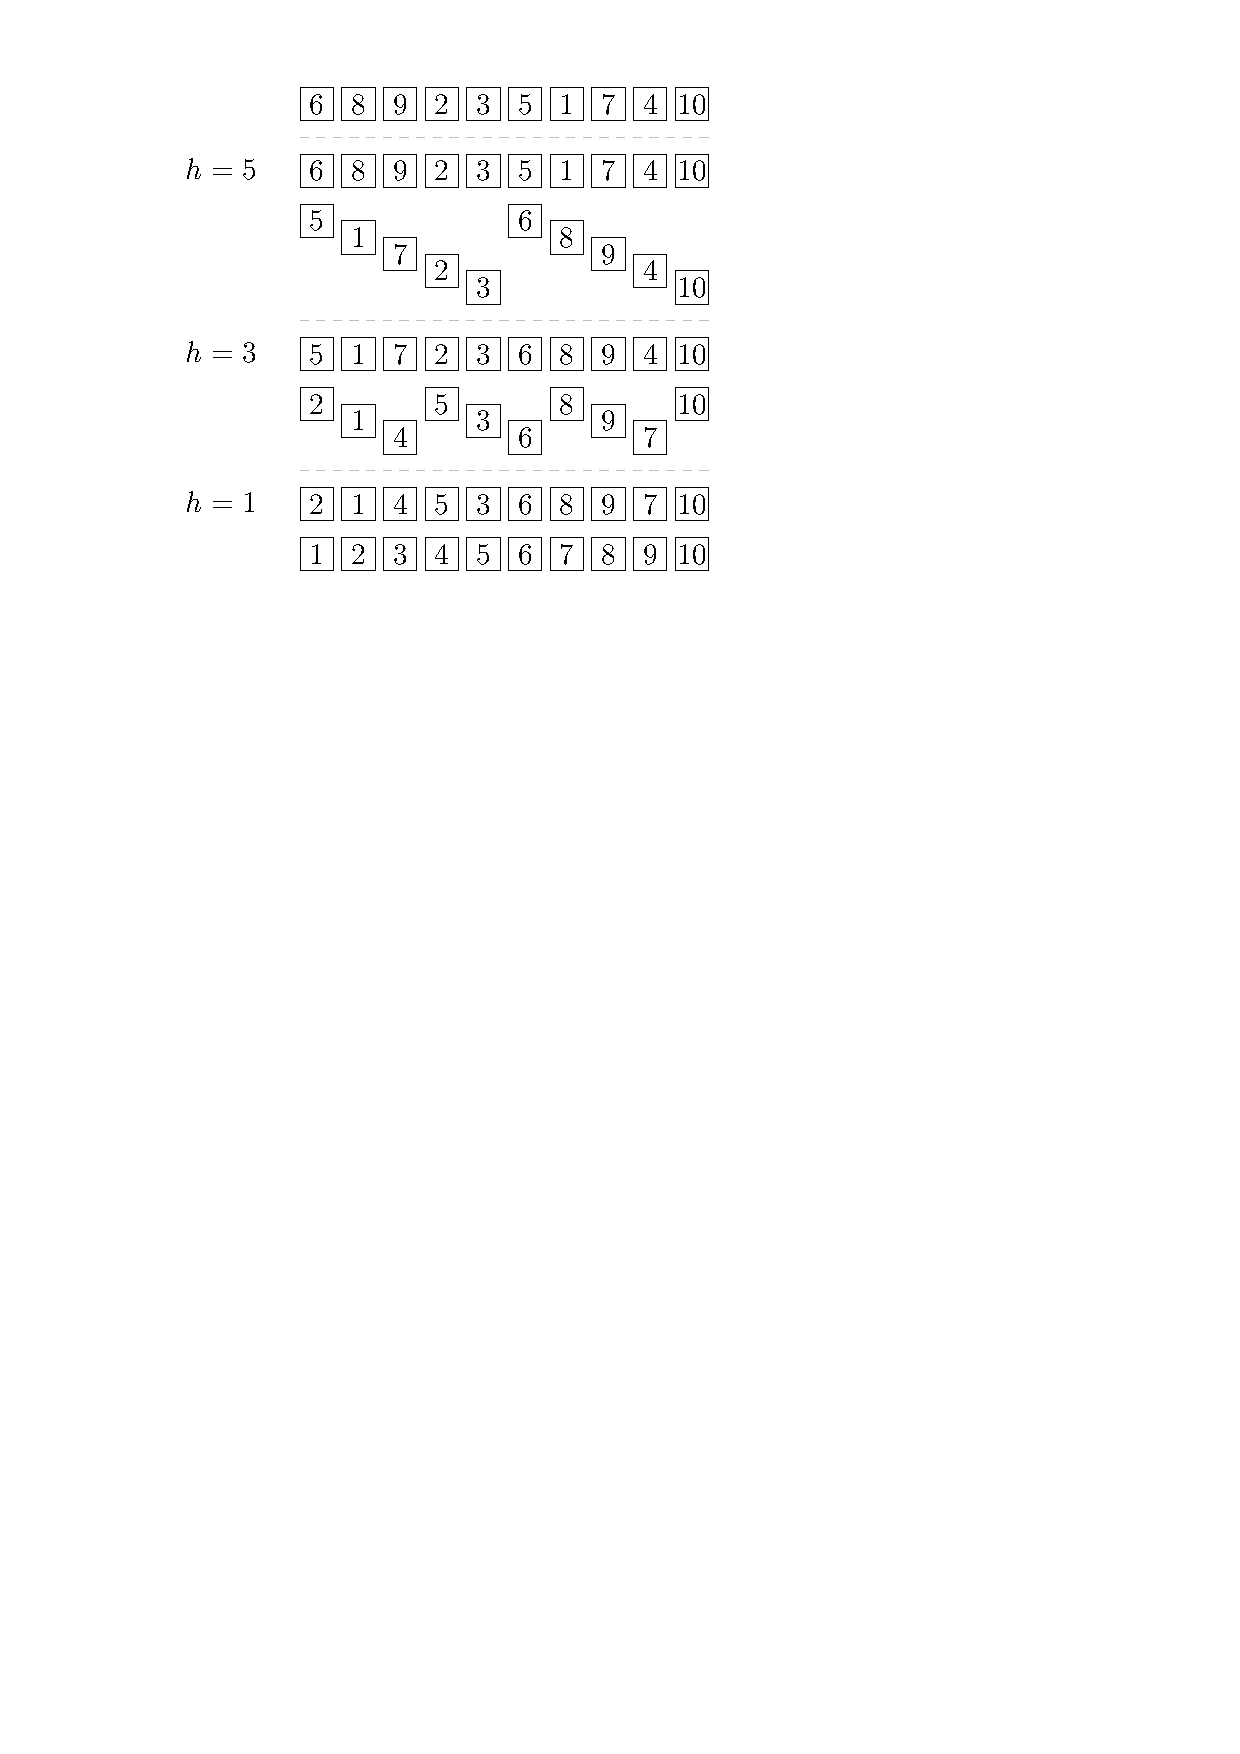
\includegraphics[width=0.55\linewidth]{ShellSort} 
\end{center}
\end{Boxample}

This is a simple algorithm whose analysis is very hard. 
Values of $h$ chosen from all relevant numbers of the form $2^i 3^j$ have been proved to give 
$O(n (\log n)^2)$ running time, but better ones are used in practice. 
Almost nothing is known about average-case running time of Shellsort. 
Empirically, behaviour that looks like $O(n^{7/6})$ has been obtained. 

Shellsort is easy to program and useful in practice for fairly large arrays (say $10^5$) especially for partially sorted data. 
It is substantially  better than insertion sort.


\chapter{Mergesort}  %----------------------------
\label{sec:mergesort}
Here we discuss two ``industrial strength" sorting algorithms,
\defnfont{Mergesort} and \defnfont{Quicksort}, and look at the first one
in more detail. 
\begin{itemize}
\item Each algorithm splits the input list into two sublists, 
recursively sorts each sublist, and then combines the sorted sublists to sort 
the original list.
\item Mergesort (J. von Neumann, 1945): splitting is very easy, most 
of the work is in combining. 
We divide the list into left and right half, and merge the recursively sorted 
lists with a procedure \texttt{merge}. 
\item Quicksort (C. A. R. Hoare, 1962): most of the work is in the 
splitting, combining is very easy. We choose a \defnfont{pivot} element, and use a 
procedure \texttt{partition} to alter the list so that the pivot is in its 
correct position relative to the left and right sublists on each side.
Then the left and right sublists are sorted recursively.
\end{itemize}
%Mergesort is stable. Quicksort is (more or less) in place. 
Each is used as the basis for 
built-in sorting algorithms in common programming languages.

\begin{algorithm}[H]
  \caption{Mergesort.}
    \label{alg:mergesort}
\begin{algorithmic}[0]
%\Require{$0 \leq i \leq j \leq n-1$}
\Function{mergesort}{list $a[0..n-1]$}
\If{$n > 1$}
\State $m \gets \lfloor (n-1)/2 \rfloor$ \Comment{median index of list}
\State $l \gets \Call{mergesort}{a[0..m]}$ \Comment{sort left half}
\State $r \gets  \Call{mergesort}{a[m+1..n-1]}$ \Comment{sort right half}
\State $a \gets  \Call{merge}{l, r}$ \Comment{merge both halves}
\EndIf
\State \Return{$a$}
\EndFunction  
\end{algorithmic}
\end{algorithm}

\section{Linear time merging for Mergesort}
The key is an efficient merge algorithm. 
If $L_1$ and $L_2$ are sorted lists, they can be merged into one sorted 
list in linear time.
\begin{itemize}
  \item Start pointers at the beginning of each list. 
  \item Compare the elements being pointed to 
  and choose the lesser one to start the sorted list. Increment that pointer. 
  \item Iterate until one pointer reaches the end of its list, 
  then copy remainder of other list to the end of the sorted list.
\end{itemize} 
If the list is implemented as an array, this merging takes linear extra 
space (cannot be done in place). But if linked lists are used, it can be done in 
place. In any case the number of comparisons is in $\Theta(n)$.

% \begin{algorithm}[H]
%   \caption{Merge.}
%     \label{alg:merge}
% \begin{algorithmic}[0]
% %\Require{$0 \leq i \leq j \leq n-1$}
% \Function{merge}{list $a[1..m]$, list $b[1..n]$}
% 	\State list $c[]$
% 	\While{$a$ is not empty and $b$ is not empty}
% 		\If{$a < b$}
% 			\State \Return $c$
% 		\EndIf
%  	\EndWhile
% \EndFunction  
% \end{algorithmic}
% \end{algorithm}

\begin{Boxample}[0]
Execute mergesort on the following input.
\begin{center}
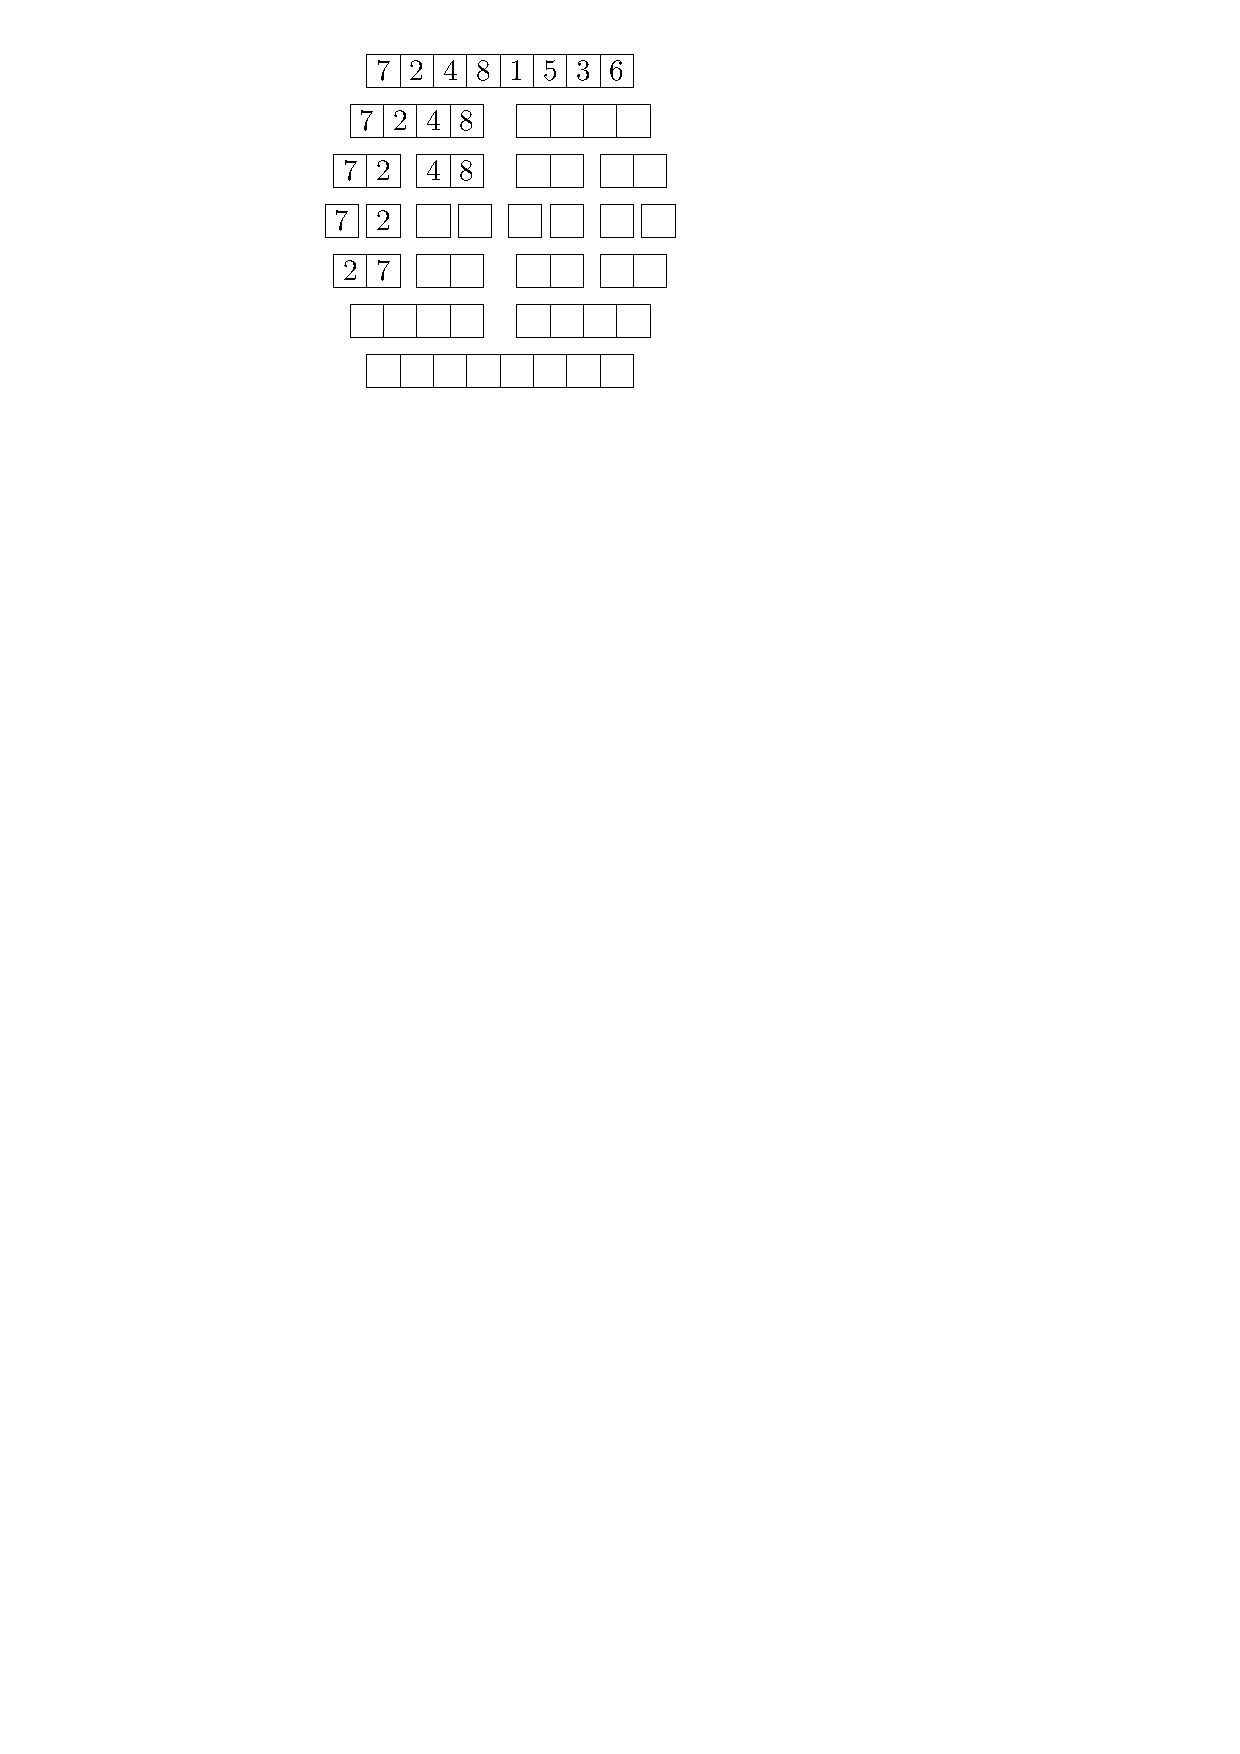
\includegraphics{MergeSort} 
\end{center}
\end{Boxample}

\section{Mergesort analysis}
The number of comparisons $C_n$ satisfies (approximately)
$$ C_n  = \left\{
\begin{array}{ll}
	C_{\lceil n/2 \rceil} + C_{\lfloor n/2 \rfloor} + n & \qquad \text{if }n > 1\text{;} \\
														0 & \qquad \text{if }n = 1\text{.}
\end{array}\right.$$
Thus if $n$ is a power of 2 we have $C_n = 2C_{n/2} + n$. We need to develop tools to solve recurrences like this --- see the next lecture.

\section{Which inputs give the best and worst case?}
Mergesort is not very sensitive to the input order. 
If the input is already sorted, the merge operation does the fewest possible comparisons. 
The worst case occurs when the input looks like 5,1,7,3,6,2,8,4 (every possible comparison is made at every level of the merge). 
However the input only affects lower order terms -- it turns out 
(next lecture)  that mergesort does about $n \lg n$ comparisons on every input.

\section{Is mergesort in-place?}
\begin{Boxample}[6]
Show by example that it is not, when implemented on an array.
\end{Boxample}

\section{Is mergesort stable?}

\begin{Boxample}[0]
Execute mergesort on the following input to convince yourself that the algorithm is stable.
\begin{center}
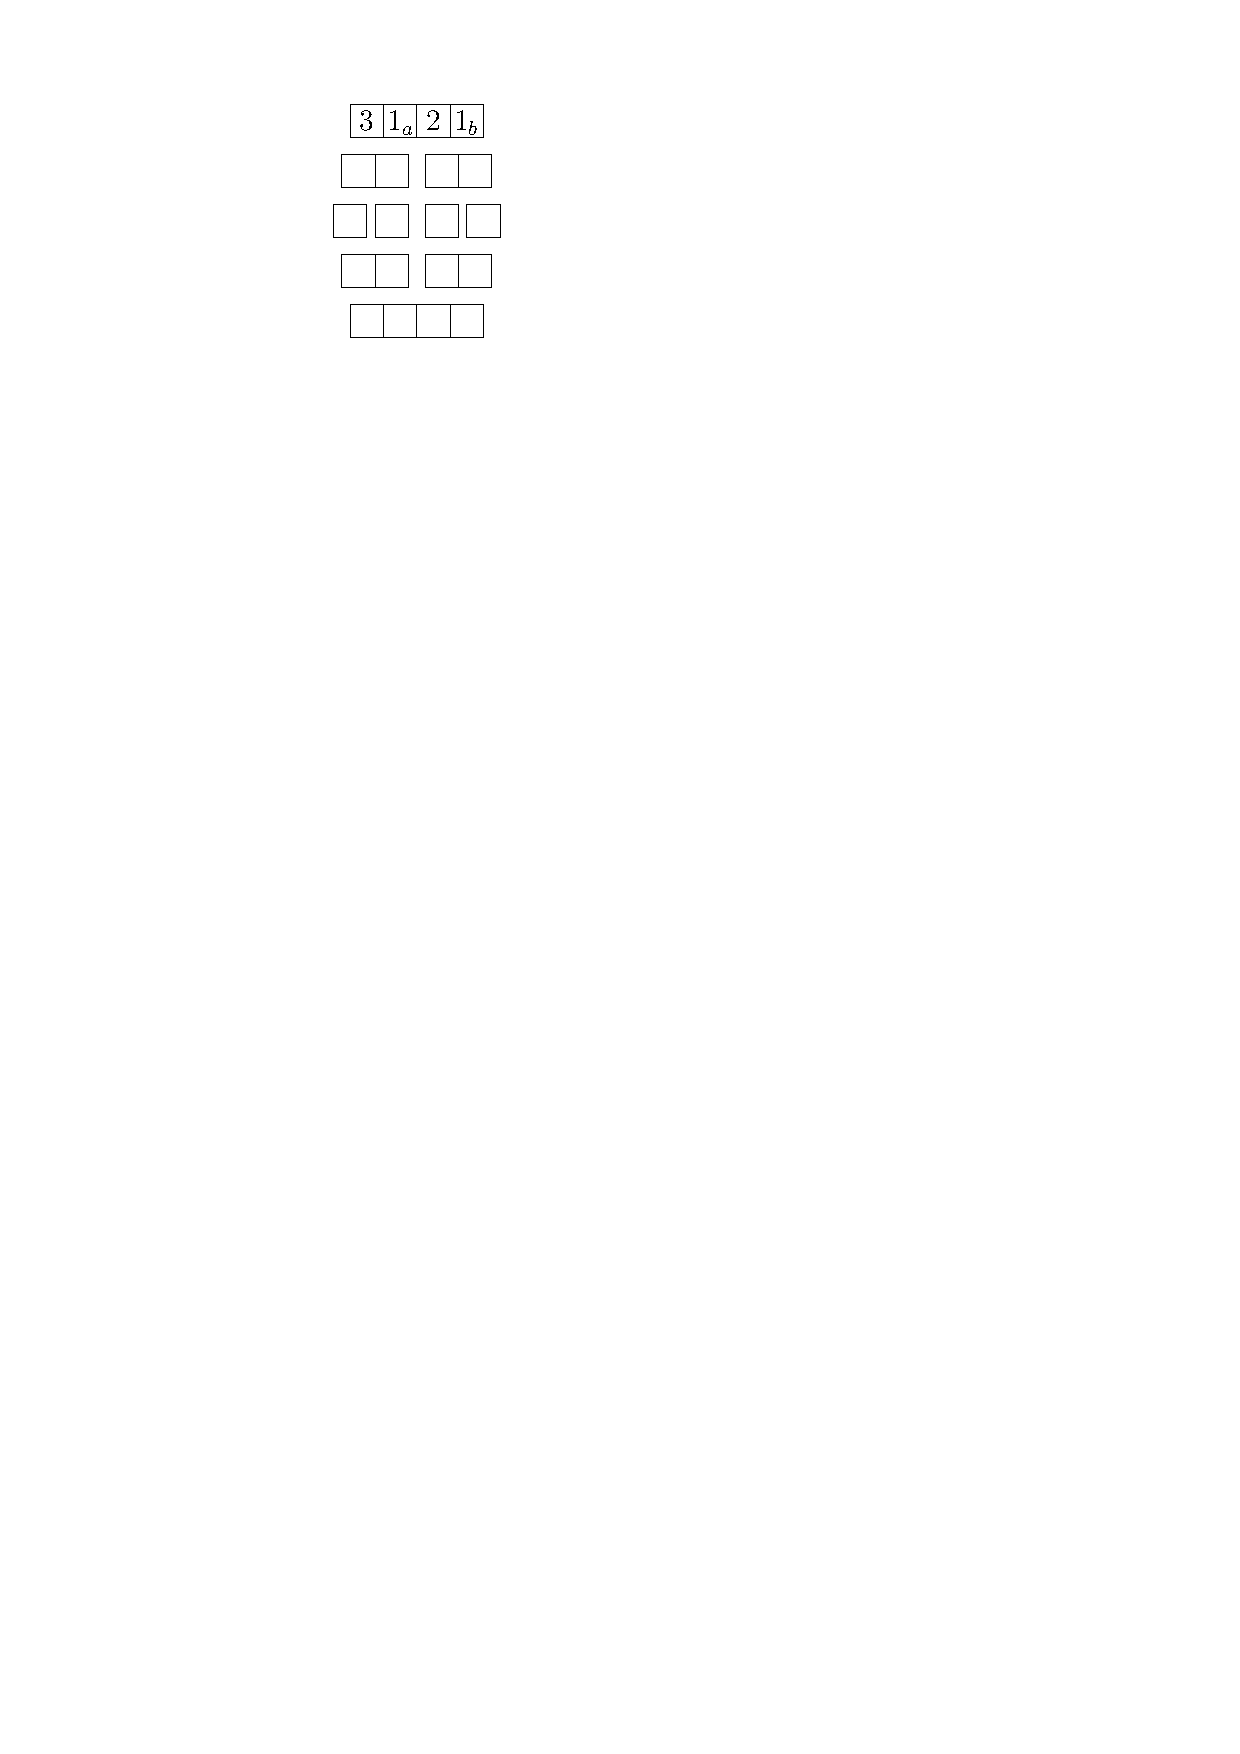
\includegraphics{MergeSortStable} 
\end{center} 
\end{Boxample}

\section{Analysis when implemented on a linked list}
Since finding the middle element of the list is time-consuming, in this case it makes more sense to ``unroll" the recursion 
and process all the instances at the bottom of the recursion tree (merging two size 1 lists) first, then merge all the resulting size 2 lists two-by-two, etc. 
This ``bottom-up mergesort" is not only equivalent to mergesort, it is in place! Note that ``bottom-up mergesort" is strictly speaking a different algorithm from mergesort.

% \begin{Boxample}[0] % mergesort with first part cut off.
% Execute  bottom-up mergesort  on the following input.
% \begin{center}
% % 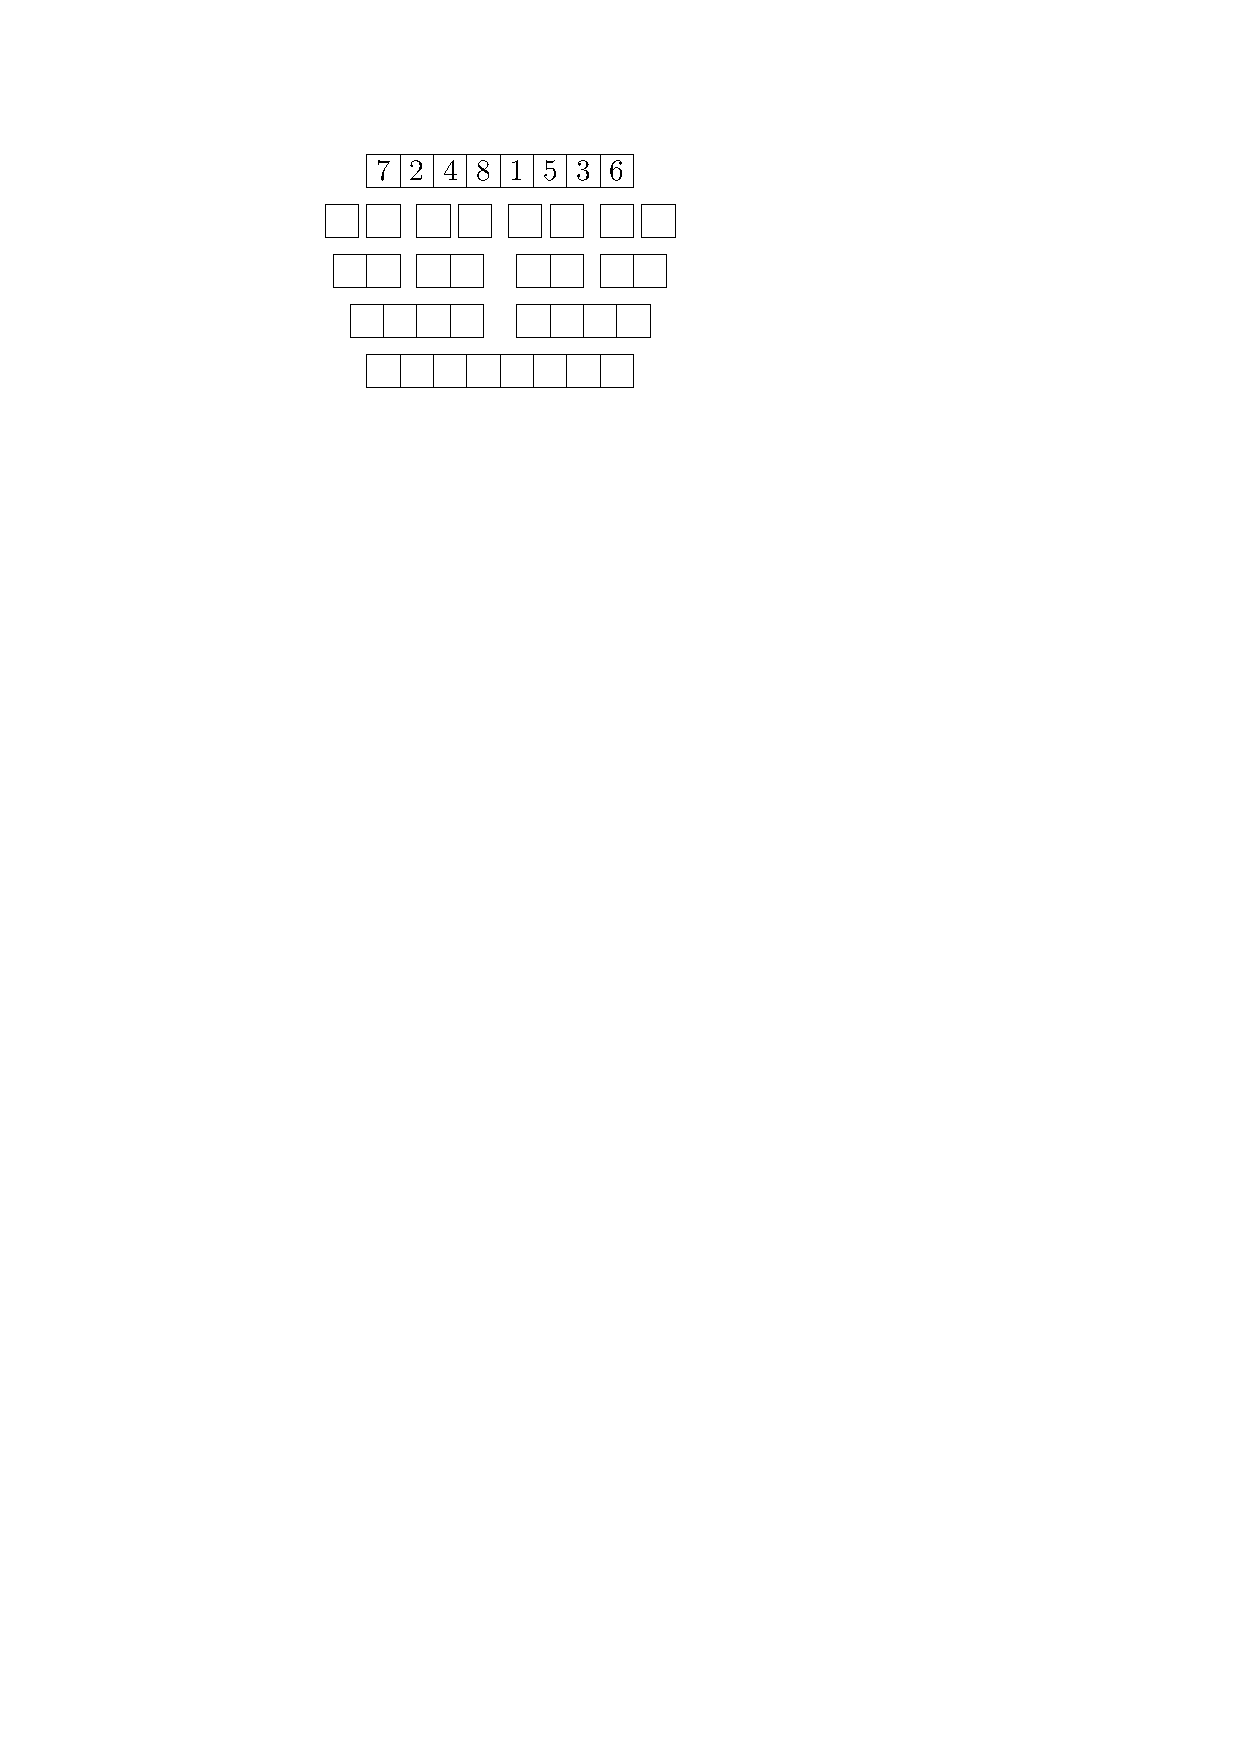
\includegraphics{MergeSortBottomUp} % version with same numbers as others, but then same as for recursive boxample
% 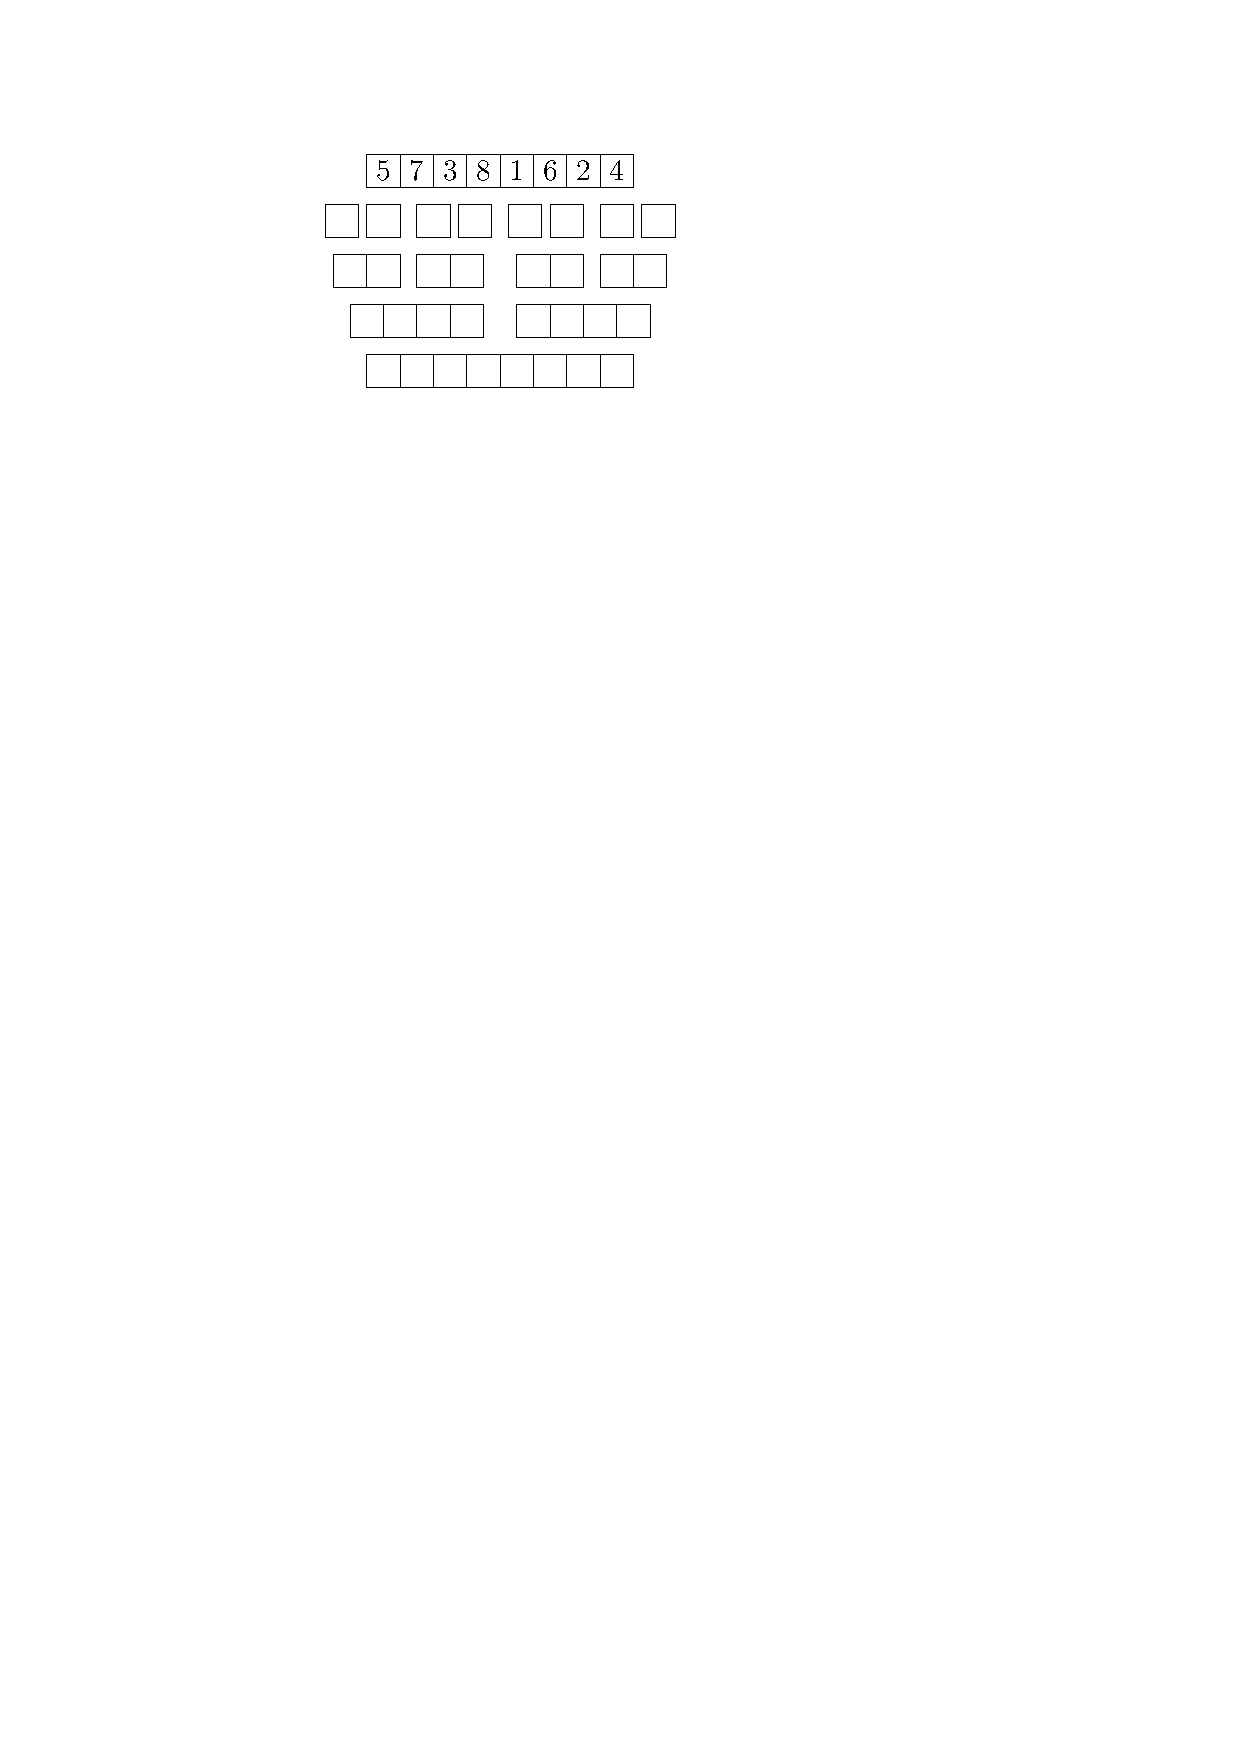
\includegraphics{MergeSortBottomUp2}
% \end{center}
% \end{Boxample}

% \frametitle{Mergesort and quicksort pseudocode}
% \begin{tabbing}
% xxxx\=xxxx\=xxxx\=xxxx\=xxxx\=xxxx\=xxxx\= \kill
% \textbf{algorithm} \texttt{mergesort} (list $a$) \\
% $n \gets size(a)$; $b \gets a[0..n/2]; c \gets a[1+n/2, \dots n-1];$ \\
% $t \gets $ \texttt{merge} (\texttt{mergesort}($b$), \texttt{mergesort}($c$)) \\
% \textbf{return} $t$ \\
% \textbf{end}
% \end{tabbing}	
% \begin{tabbing}
% xxxx\=xxxx\=xxxx\=xxxx\=xxxx\=xxxx\=xxxx\= \kill
% \textbf{algorithm} \texttt{quicksort} (list $a$, integers $l, r$) \\
% $n \gets size(a)$; $p \gets$ \texttt{pivot}($a$)\\
% $i \gets \texttt{partition}(a, p)$ \quad \{puts $p$ in right place\} \\
% \texttt{quicksort}($a[l..i-1]$); \texttt{quicksort}($a[i+1..r]$)\\
% \textbf{end}
% \end{tabbing}


\chapter{Recurrences} %-------------------------------------------------------
\begin{Definition}
A \defnfont{recurrence relation} or \defnfont{difference equation} is an
equation that defines an unknown function $F$ recursively. 
The value $F(n)$ is determined by the values $F(0), F(1), \dots, F(n-1)$ for
sufficiently large $n$. The smaller values of $n$ are called the
\defnfont{initial conditions}. 
\end{Definition}

\section{Important special cases}
\begin{description}
  \item[Tower of Hanoi:] $T(n) = 2 T(n - 1) + 1$, $T(1) = 0$.
  \item[Searching a linked list:] $T(n) = T(n - 1) + 1$, $T(0) = 0$.
  \item[Insertion sort:] $T(n) = T(n-1) + n$, $T(0) = 0$.
  \item[Binary search:] $T(n) = T(n/2) + 1$, $T(1) = 0$ makes sense when $n$ is a power of $2$. 
  \item[Mergesort:] $T(n) = 2T(n/2) + n$, $T(1) = 0$ makes sense when $n$ is a power of $2$.
  \item[Quicksort:] $T(n) = (2/n)\sum_{i<n} T(i) + n-1$, $T(1) = 0$.
\end{description}

Important examples  in this course are \defnfont{constant coefficient linear recurrences} which have the form 
$F(n) = \sum_{k=1}^K a_k F(n - k)$ for some fixed $K$ and some constants $a_k$. 
Examples are the Fibonacci numbers, $F(n) = F(n-1) + F(n-2)$ and the power of $2$, $F(n) = 2F(n-1)$.

We deal with only two easy techniques here: ``bottom-up" and ``top-down" guessing. 
In each case we guess a pattern and (should) prove it by mathematical induction. 
Sometimes a simple change of variable can convert a more difficult-looking recurrence into an easy one. 

\section{Top-down solution method example}
\begin{Boxample}
We are given $T(n) = 2 T(n - 1) + 1, T(1) = 0$. We can iterate this to obtain 
\begin{align*}
T(n) & = 2 T(n - 1) + 1  \\
& = 2 [2 T(n - 2) + 1] + 1 = 2^2 T(n-2) + (2 + 1) \\
& = 2^2 [2T(n - 3) + 1] + (2 + 1) = 2^3 T(n - 3) + (2^2 + 2+ 1)  \\ 
& = \dots = 2^{n-1} T(1) + (2^{n-2} + \dots + 2 + 1)  \text{ if $n \geq 1$} \\
& = \sum_{0\leq i < n-1} 2^i = 2^{n-1} - 1\text{.}
\end{align*}
\end{Boxample}

\section{Bottom-up solution method example}
\begin{Boxample}
We are given $T(n) = 2 T(n - 1) + 1$, $T(1) = 0$. 
We compute values from the bottom up using the recurrence.\\


We have $T(1) = 0$, $T(2) = 2T(1) + 1 = 1$, $T(3) = 2T(2) + 1 = 3$, $T(4) = 7$, $T(5) = 15$. 

We guess $T(n) = 2^{n-1} - 1$. The guess is correct when $n = 1$.
Now assume that $n > 1$ and the formula holds for all smaller values than $n$. 
From the recurrence we then have 
$T(n) = 2T(n-1) + 1 = 2(2^{n-2} - 1) + 1 = 2^{n-1} - 1$. 
Thus the formula holds for all $n \geq 1$, by \boldfont{mathematical induction}.
\end{Boxample}

\section{Change of variable}
\begin{Boxample} \label{eg:recur-cov}
Consider the divide-and-conquer recurrence $T(n) = T(n/2) + 1$, $T(1) = 0$. 
This makes sense for $n$ a power of $2$.\\

Changing variable by $n = 2^i$, $T(n) = U(i)$ 
gives $U(i) = U(i-1) + 1$, $U(0) = 0$. 
By top-down or bottom-up guessing as above, we get 
$$T(n) = U(i) =  i = \lg n$$ when $n$ is a power of $2$.

Similarly the mergesort recurrence $T(n) = 2T(n/2) + n, T(1)  = 0$ 
has solution $T(n) = n \lg n$ for $n$ a power of $2$.
\end{Boxample}

\begin{Boxample}[6]
How does the solution to \cref{eg:recur-cov} look if we do not do the change of variable?
\end{Boxample}

\section{Mathematical extra: dealing with floors and ceilings, etc}
The mergesort recurrence involves floor and ceiling functions. How do we deal with these?

We can solve the mergesort recurrence $T(n) = T(\lceil n/2 \rceil) + T(\lfloor n/2 \rfloor) + n$ asymptotically. 
``Exact" solutions are hard. See COMPSCI 720 and beyond. Then we consider the recurrence $\hat{T}(n) =
2\hat{T}(\lceil(n/2)\rceil) + n$. It is easily shown that $T \leq \hat{T}$, and 
as above $\hat{T}(n) = n \lg n$ for $n$ a power of $2$. We can then show that $T(n)$ is $O(n \lg n)$. A similar argument gives $T(n)$ is $\Omega(n \lg n)$.

In real life we usually do not have exactly an additive term $n$
but just some $f(n)$ where $f(n)$ is $\Theta(n)$. Similar techniques show that 
we get the same answer, asymptotically. 


\section{How do we solve the Fibonacci recurrence?}
Recall $F(0) = 0$, $F(1) = 1$, $F(n) = F(n-1) + F(n-2)$,  $(n \geq 2)$.
Such linear homogeneous recurrences can be solved exactly with
more theory than we have time for in this course. 

\begin{Boxample}[3]
Try to solve the Fibonacci recurrence using the top-down or bottom-up method. Why does it fail?

\end{Boxample}

To find an asymptotic solution for $F(n)$ (which is all we need here), we conjecture, based on examples, 
that $F(n)$ grows exponentially in $n$. 
In other words, there are $C > 0$ and $r > 1$ such that 
$F(n) \geq C r^n$ for all sufficiently large $n$.

Try to prove this by induction. The obvious method gives 
$F(n+1) = F(n) + F(n-1) \geq C(r^n + r^{n-1}) = Cr^{n}(1+r)$, so that we easily obtain
the conclusion we want if and only if $1 + r \geq r^2$, or $r \leq
\phi:= (1 + \sqrt{5})/2 \approx 1.618$. 

Now suppose $F(n) \leq D r^n$ for all sufficiently large $n$. 
Trying to prove this by induction, we require $1 + r \leq r^2$ or $r \geq \phi$. 

Thus $F(n)$ is $\Theta(\phi^n)$.


\chapter{Quicksort} %---------------------------------------------------------
\label{sec:quicksort}

\defnfont{Quicksort} was described briefly in \cref{sec:mergesort}. We give the details now. Note that a purely recursive version would do a lot of copying to 
create new versions of the left and right sublists, as happens with mergesort. In terms of programming languages, we are talking about ``passing by value". 
We can get an in-place implementation if we use functions that can modify the value of their argument without explicitly returning them 
(they have ``side effects", usually implemented in programming languages via ``passing by mutable reference", which is commonly done for arrays by default).

\begin{algorithm}[H]
  \caption{Quicksort - basic.}    
  \label{alg:quicksort}
\begin{algorithmic}[0]
	\Require{$0 \leq i \leq j \leq n-1$}
	\Comment{Side effect: changes $a$}
	\Function{quicksort}{list $a[0..n-1]$, integer $i$, integer $j$} 
		\If{$i < j$}
		        \State $q \gets  \Call{partition}{a, i,j}$ \Comment{put pivot in correct position}
			\State $\Call{quicksort}{a,i,q-1}$ \Comment{sort left half}
			\State $\Call{quicksort}{a,q+1,j}$ \Comment{sort right half}
		\EndIf
	%\State \Return{$a$}
	\EndFunction  
\end{algorithmic}
\end{algorithm}

The exact way in which quicksort works depends on the details of the way we choose the pivot element and how the 
partition algorithm works. Each choice for these gives a different quicksort algorithm.
We use the first entry as pivot element for a basic presentation, but there are better options in practice.

\begin{Boxample} \label{ex:quicksortSmall}
Illustration of quicksort. First the array is partitioned and the pivot element 4 moved into the middle. 
Then the left side (``$< 4$'') and right side (``$> 4$'') are recursively sorted.
\begin{center}
  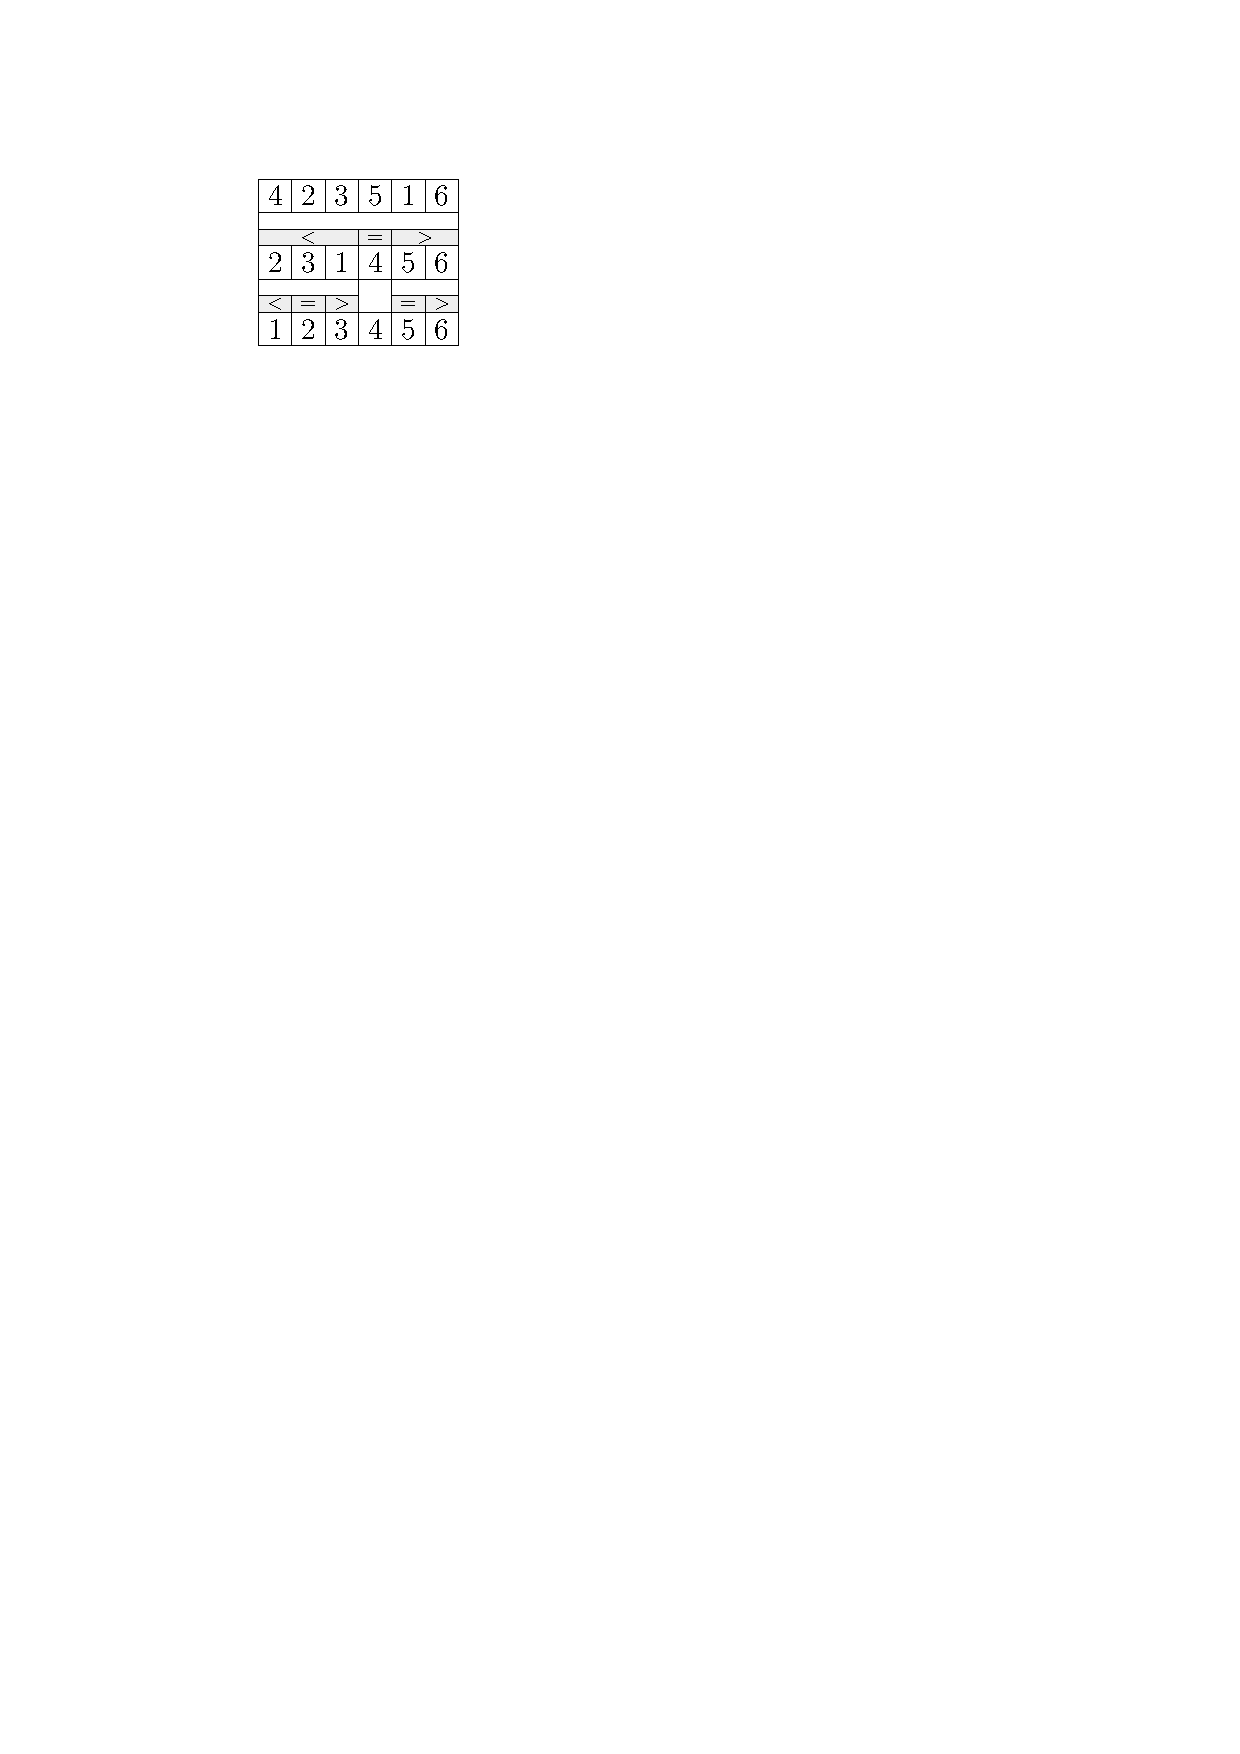
\includegraphics{QuickSortExampleDifPartition}
\end{center}
\end{Boxample}


\section{Linear time partitioning}
Given a list $L$ and an element $p$ of $L$ called the pivot, we can partition so
 that all elements to the left of $L$ are $\leq p$ and all to the right are 
$\geq p$. One method is \cref{alg:partition} (Hoare, 1960) and it works as follows.
\begin{itemize}
\item Start with pointers at opposite ends of the list. Stop when pointers cross.
\item At each step, increment the left pointer until we reach an element $\geq p$, and decrement the right one until we reach an element $\leq p$. 
\item Swap these elements and continue. When pointers cross, swap right pointer with pivot.
\end{itemize}

\begin{algorithm}[H]
  \caption{Partition - Hoare's method.}
    \label{alg:partition}
\begin{algorithmic}[0]
\Require{$0 \leq i \leq j \leq n-1$}
\Comment{Side effect: changes $a$}
\Function{partition}{list $a[0..n-1]$, integer $i$, integer $j$}
	\State $p \gets a[i]$ \Comment{pivot element}
	\State $l \gets i $ \Comment{left pointer}
	\State $r \gets j+1$ \Comment{right pointer}
	\While{True}
		\Repeat
			\State $l \gets l+1$ \Comment{find big element}
		\Until{$a[l]\geq p$} 
		\Repeat
			\State $r \gets r-1$ \Comment{find small element}
		\Until{$a[r] \leq p$} 
		\If{$l < r$}
			\State \texttt{swap}$(a,l,r)$  \Comment{swap big and small elements}
		\Else
			\State \texttt{swap}$(a,i,r)$  \Comment{put pivot in correct place}
			\State \Return{$r$}
		\EndIf
	\EndWhile
\EndFunction  
\end{algorithmic}
\end{algorithm}


\begin{Boxample}[0]
Complete the following example for the partition algorithm \cref{alg:partition}. 
Begin with setting the pointers $p$, $l$ and $r$ after finding the big and small element in the second iteration.
\begin{center}
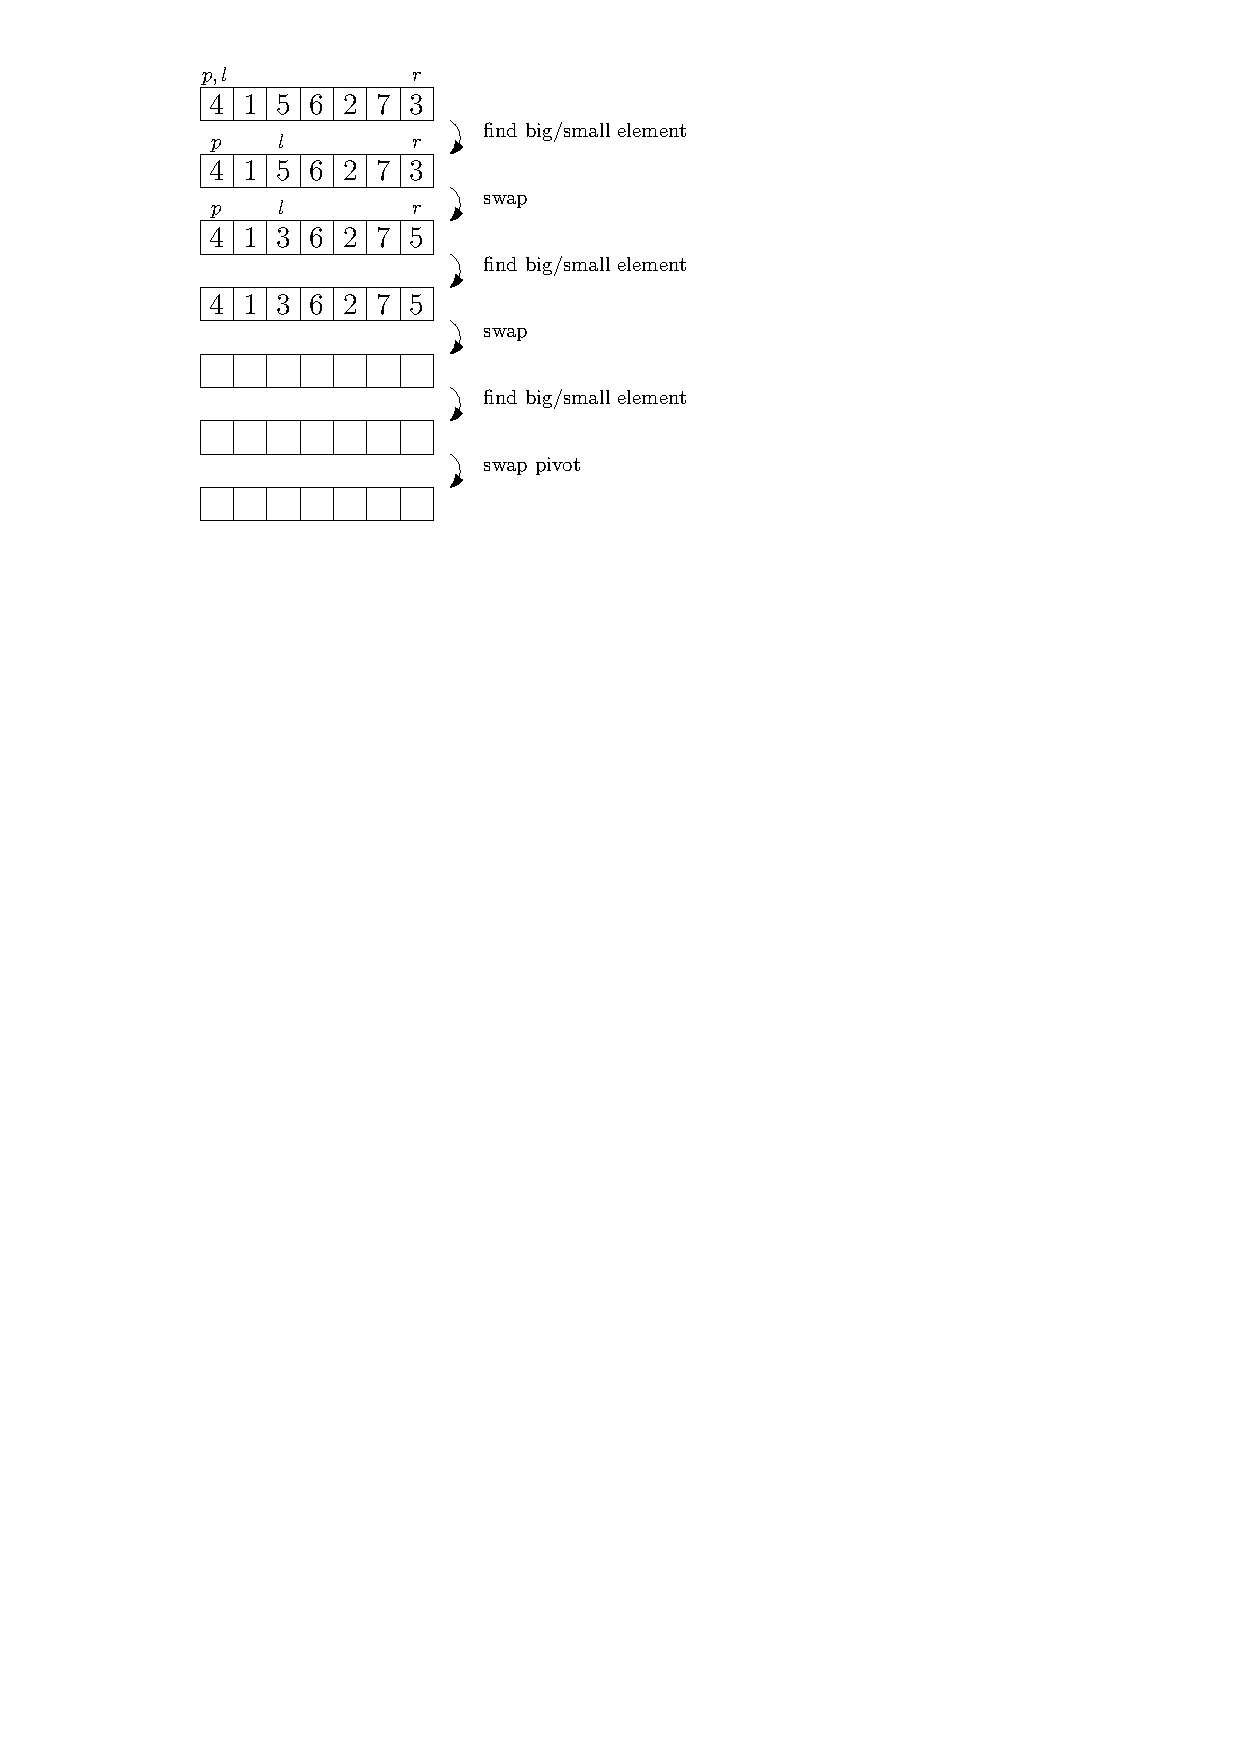
\includegraphics{partitionAlgo}
\end{center}
\end{Boxample}

\begin{Boxample}[1]
Does the quicksort algorithm in \cref{ex:quicksortSmall} use Hoare's method, \cref{alg:partition}, for partitioning? 
\end{Boxample}


\begin{Boxample}[2]
Execute the quicksort algorithm \cref{alg:quicksort} using Hoare's partition algorithm.
\begin{center}
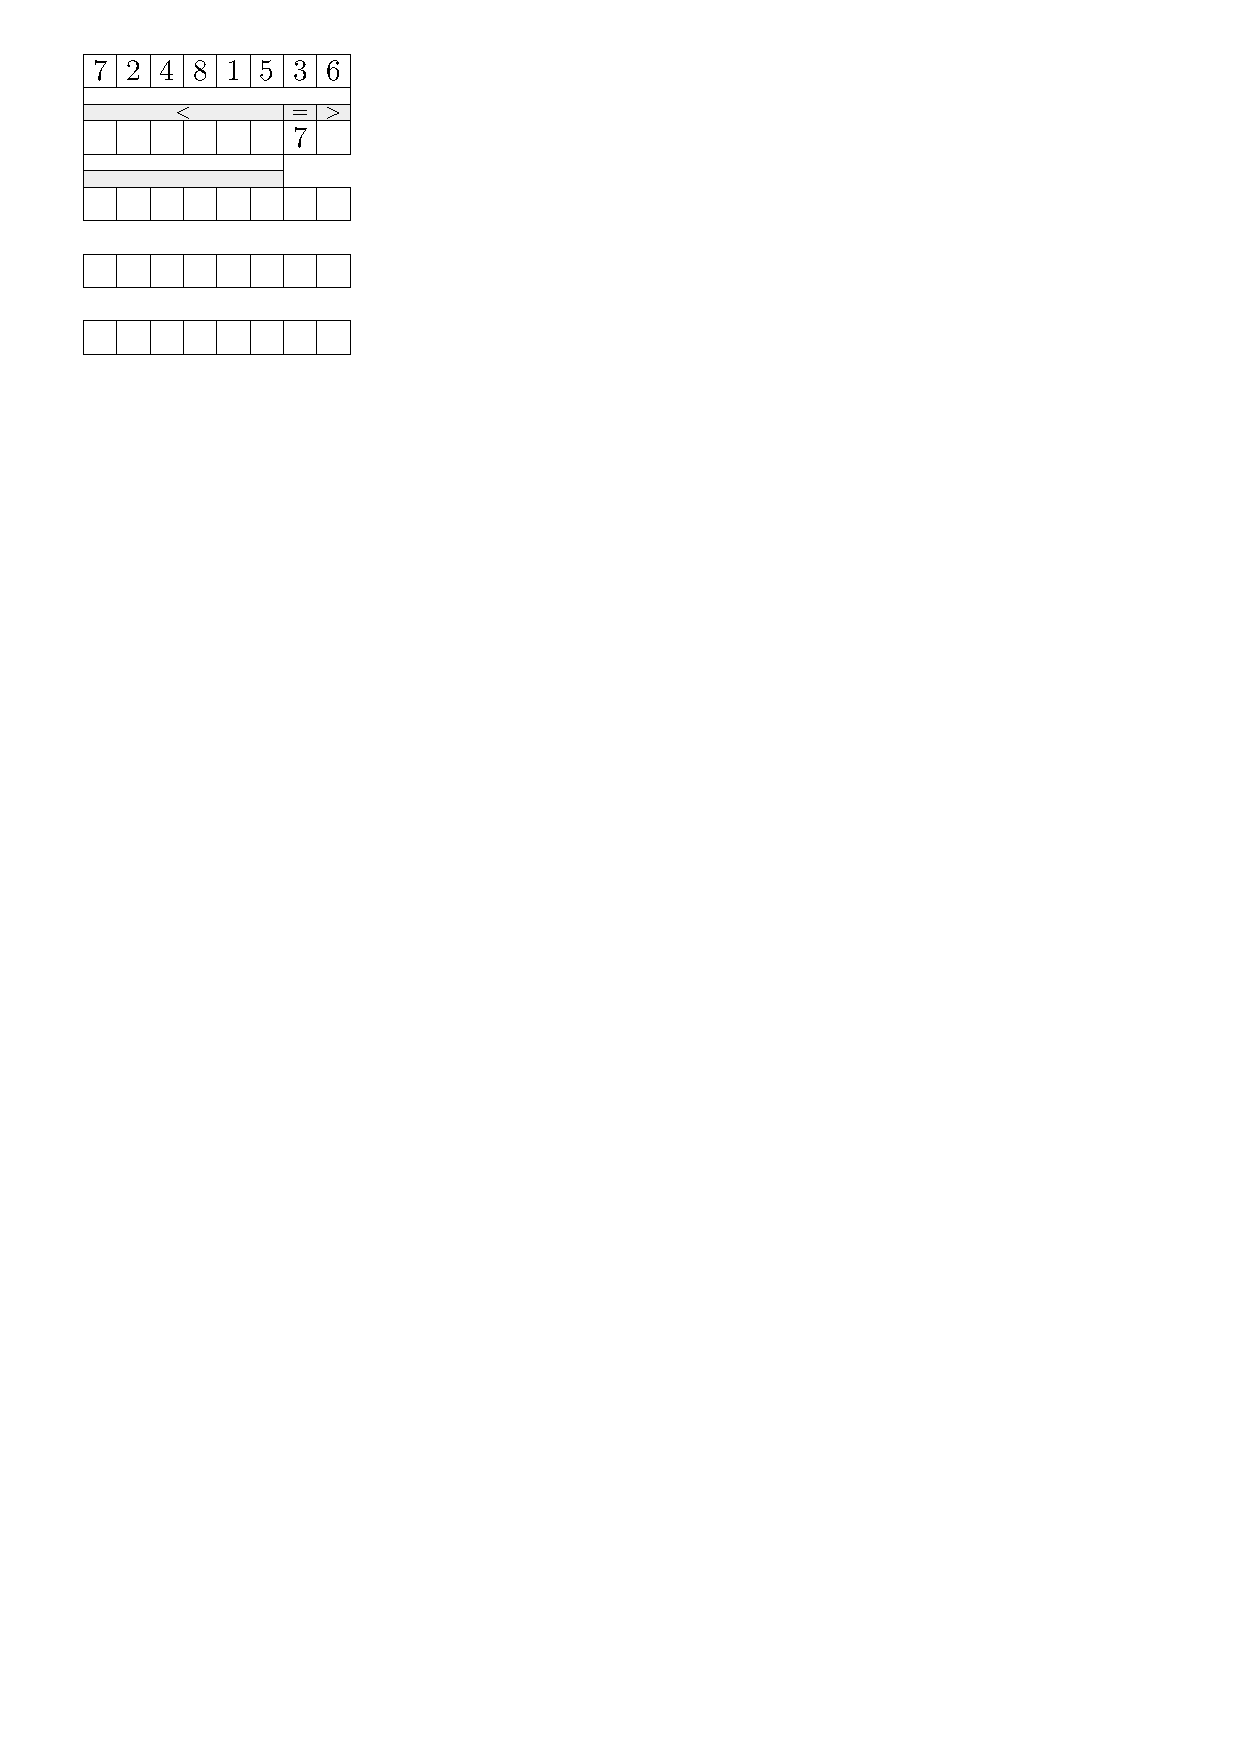
\includegraphics{QuickSortExercise}
\end{center}
\end{Boxample}

\section{Quicksort analysis}
The number of comparisons satisfies a recurrence like 
$C_n = C_{p-1} + C_{n - p} + n$. If we are unlucky (like when the list is already sorted), this degenerates to 
$C_{n} = C_{n-1} + n$ and we get quadratic running time.

However, quicksort seems to behave well in practice. We can prove that 
if elements are distinct and all input permutations are equally likely, then 
quicksort has average running time in $O(n \log n)$.

The recurrence for this average running time is basically
$$ a_n = \frac{2}{n} \sum_{i<n} a_i + n-1. $$ 
This requires a different solution method to the easier recurrences.
%\item  Answer turns out to be $a_n = 2 (n + 1) H_n - 4n$ we know 
%that $H_n$ is $\Theta(\log n)$.

\section{Quicksort recurrence solution}
Let $a_n$ be the average of $C_n$ so that 
$a_n = n - 1 + \frac{1}{n} \sum_{1\leq p \leq n} (a_{p-1} + a_{n-p})$. 
Collect common terms in the sums to obtain
$$a_n = n - 1 + \frac{2}{n} \sum_{j=0}^{n-1} a_j.$$ 
Note that to compute each term using this recurrence, we require knowledge of all previous terms.
We first \emph{eliminate the history}, (a general form of \emph{telescoping}). 
%\item The solution is 
%$a_n = 2 (n + 1) H_n - 4n \approx 2 n \ln n$, where 
%$$H_n:= \sum_{1\leq j \leq n} 1/j.$$ 

We have for $n>1$
\begin{align*}
na_n - (n-1) a_{n-1} & = n(n-1) + 2 \sum_{0\leq j < n} a_j \\
& - (n-1)(n-2) - 2\sum_{0 \leq j < n - 1} a_j \\
& = 2(n - 1) + 2 a_{n-1}\text{.}
\end{align*}
Thus $na_n = 2(n - 1) + (n+1)a_{n-1}$, so that 
$$
\frac{a_n}{n+1} = \frac{2(n-1)}{n(n+1)} + \frac{a_{n-1}}{n} = 
\frac{a_{n-1}}{n} + \frac{4}{n+1} - \frac{2}{n}\text{.}
$$
We can iterate to obtain
$$\frac{a_n}{n+1} = \frac{a_1}{2} + \sum_{j=2}^n \left(\frac{4}{j+1} - 
\frac{2}{j}\right) = 4(H_{n+1} - (1+1/2)) - 2(H_n - 1)\dots = 2H_n + \frac{4}{n+1} - 4\text{.}$$

\section{Which inputs give the best and worst-case?}
The worst case number of comparisons occurs when the pivot is always at the end of the sublist. 
For example, if we always choose the first element as the pivot and the input is in sorted order, this will happen. 
The running time is then $\Theta(n^2)$. 
The best case occurs when the pivot turns out to be the median element, so that the left and right subarrays are balanced at each level of the recursion, 
and this gives running time in $\Theta(n\log n)$ as with mergesort.

\section{Is quicksort in-place?}
Not technically, but almost. It requires $\Theta(\lg n)$ space for the recursion stack. This is very little extra space in practice, but it is not a constant amount.

\section{Is quicksort stable?}
No.
\begin{Boxample}[5]
Create an example that shows that quicksort is not a stable sorting algorithm.
\end{Boxample}

\section{What happens if we  use quicksort on a linked list?}
Although it could be done, quicksort is almost never used on a linked list. It is too difficult to quickly find a good pivot element, for example.

\section{How can we improve quicksort?}
If we always choose the first element of the list as the pivot, it is easy to implement but
the worst-case runtime is $\Omega(n^2)$, and it is easy for a malicious adversary to submit input 
which will trigger this behaviour. This naive choice (the first one used by Hoare) is very rarely used any more.

For a better way of choosing the pivot, we can take the median of a sample of (say 3) elements. This reduces the 
likelihood of worst-case behaviour and also makes performance on sorted arrays 
and arrays with equal keys better. 

Choosing a pivot element uniformly at random (or randomly shuffling the list and choosing the first element) 
gives a \boldfont{randomized} 
algorithm whose expected running time on every input can be proved to be in 
$O(n \log n)$. 

No matter how we choose the pivot as above, there is always some chance of quicksort running in quadratic time. 
Choosing the exact median turns out to be too time-consuming: see \cref{sec:qselect}.

It is best to use insertion sort once the sublists become very small, to 
avoid excessive overhead owing to recursion. 
Choosing the cutoff point requires more detailed analysis; somewhere around 10 is often used. 
This idea can be used with any recursive sorting algorithm.


\chapter{Lower complexity bound for sorting} %--------------------------------
\label{sec:lowerbound}
We have seen that various algorithms do different amounts of work on different inputs, 
and their best and worst case inputs are different in general.

\begin{Boxample}
How many comparisons do selection sort, insertion sort, mergesort, quicksort do on the following input?
\begin{center}
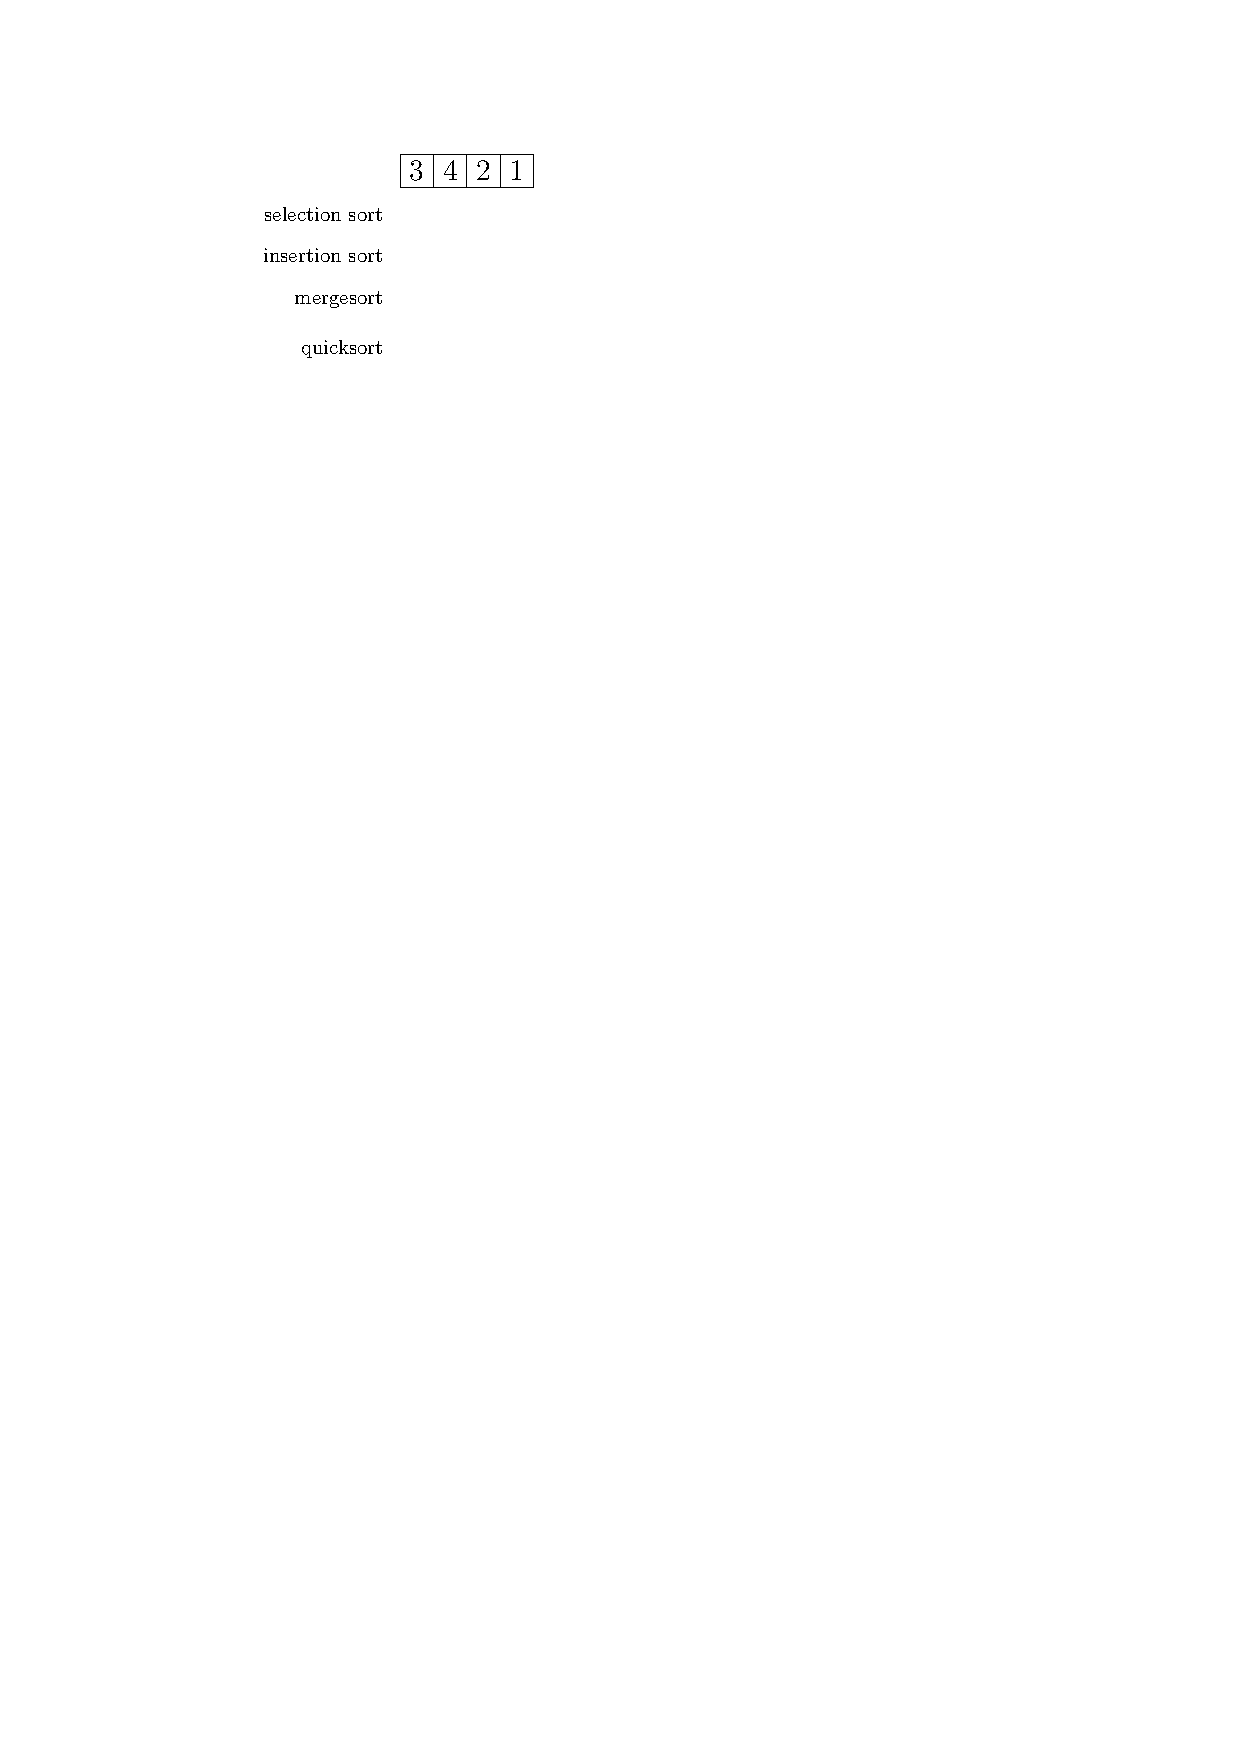
\includegraphics{numberOfComparisons}
\end{center}
\end{Boxample} 

Is it possible to sort $n$ items in $O(n)$ time in the worst case? 
Is there a general sorting algorithm $A$ and constant $c>0$ such that for all inputs of size $n$, 
$A$ uses at most $cn$ comparisons to sort? Interestingly, the answer is no, as we shall now see.

Let $\algo$ be a comparison-based sorting algorithm. 
The execution of $\algo$ on an input of $n$ distinct keys can be modelled by a \defnfont{decision tree}. 
This is a binary tree whose leaves are the $n!$ possible permutations of the keys. 
At each step we can only ask a Yes/No question of the form ``$(a_i < a_j)$?'', and this determines the branching: 
left for Yes, right for No. 
The number of comparisons required to obtain the output at a leaf is the 
length of the path from the root to that leaf (the depth of the leaf node). 
Thus the worst case number of comparisons is the maximum depth (the height) of the tree.

\begin{Boxample}
Here is the decision tree for selection sort when run on an  input list of size $3$. The label 
``$i$ vs $j$" means that the $i$th element of the input list is compared to the $j$th element, by asking
``is $a[i] < a[j]$?"
\begin{center}
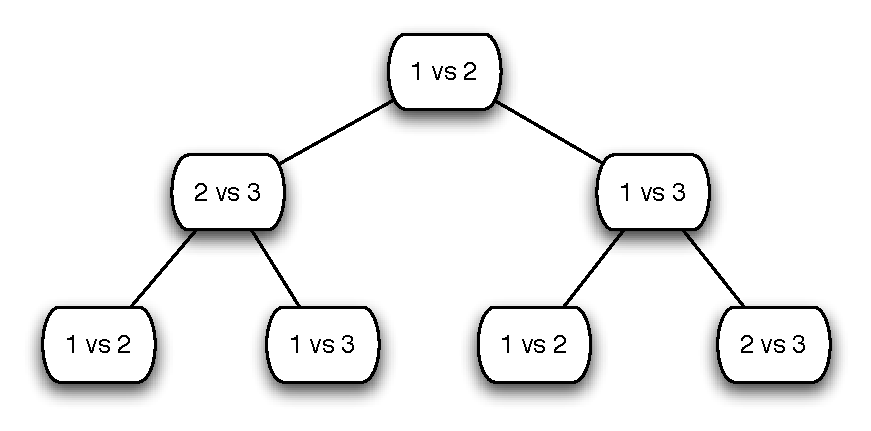
\includegraphics[width=8cm]{figs/selsort-dt}
\end{center}

The next figure shows the corresponding decision tree for insertion sort. 
We add in the grey background nodes to give information about 
which input yields which sequence of comparisons.
\begin{center}
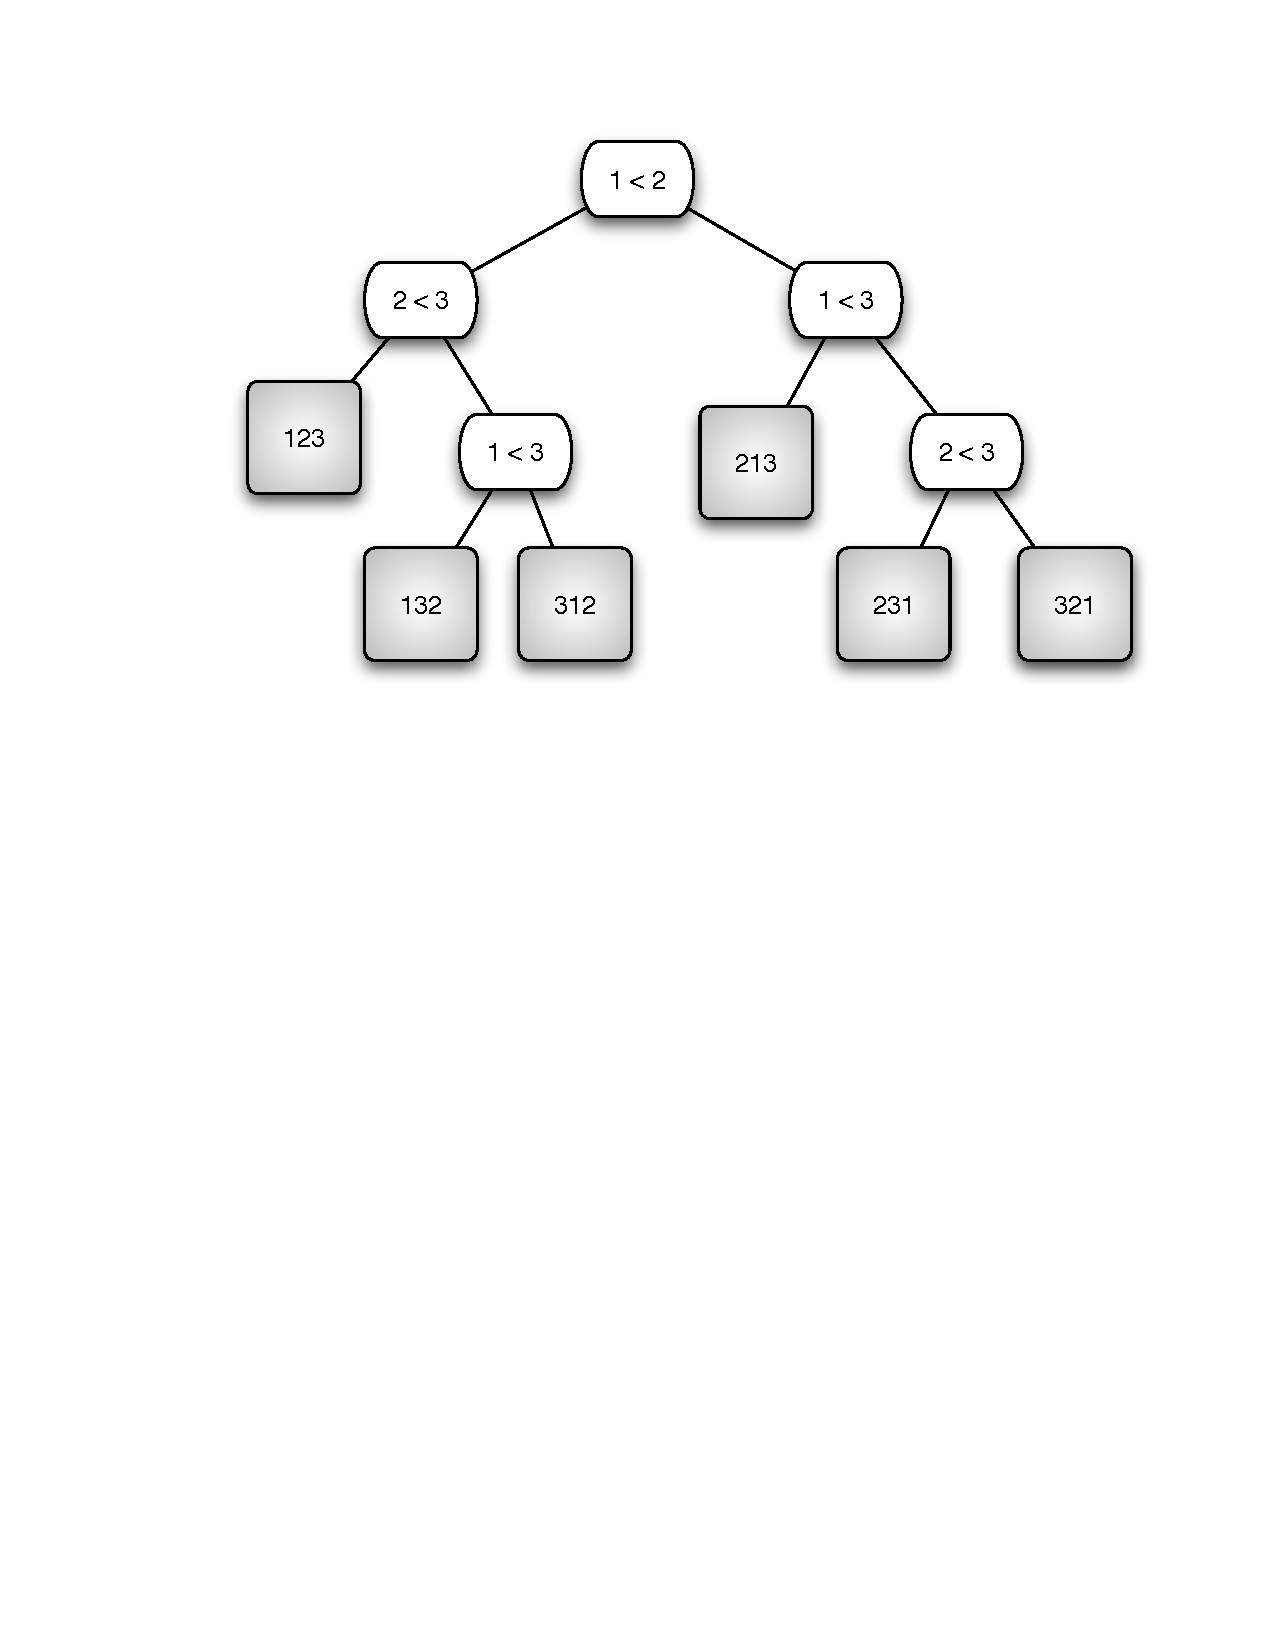
\includegraphics[width=9cm]{figs/insort-dt}
\end{center} 
\end{Boxample}

\section{Worst case height of binary decision tree} 
So, what can be said about the height of a binary tree with 
$n$ nodes?

Suppose that $T$ is a binary tree with $n$ nodes. 
Going from the root, the number of nodes at each level at most doubles.
So if the maximum depth (height) is $h$ then the number of leaves is at most $2^h$. 

In our sorting decision tree we have $n!$ leaves. 
Thus we must have $2^h \geq n!$ and therefore $h \geq \lg n!$. 

\section{Worst case running time of comparison-based sorting algorithm}
We have already shown that $\log n!$ is $\Omega (n \lg n)$. Thus the 
worst-case number of comparisons of any comparison-based sorting method must 
grow at least at the asymptotic rate $n \log n$ (any input that had duplicates 
could only make the worst case worse!)
%\item The same type of argument also works on average provided the $n!$ inputs 
%are equally likely (see textbook).  So the average-case runtime for any such 
%algorithm is  $\Omega(n \log n)$.

\begin{Boxample}[4]
We showed that the worst case for any sorting algorithm is in $\Omega (n \lg n)$. What about the average case?
\end{Boxample}

\begin{Boxample}[2]
Radix sort can sort $n$ strings in time in $\Theta(n)$.
What can we conclude about radix sort? Look it up and check your guess.
\end{Boxample}



\chapter{Priority queues and heapsort} %-------------------------------------------------
\label{sec:heapsort}
In selection sort, finding the minimum of $a[i..n-1]$ by sequential search is slow, 
and it dominates the running time. 
Can we do this operation faster? Not with the current data structure. 
We want a data structure that allows us to find and extract the minimum quickly. 
This will have applications to problems other than sorting.

\section{Priority queues}
\begin{Definition}
A \defnfont{priority queue} is a container ADT where each element 
has a key (from a totally ordered set, as with sorting) called its priority. There are operations allowing us to insert an 
element, and to find and delete the element of highest priority. 
\end{Definition}

Priority queues are important in many areas: discrete event simulation, 
graph algorithms (later in this course), sorting, \dots .
Priority queues can be implemented in many ways: unsorted list, sorted 
list, binary heap, binomial heap, \dots . 

\begin{Boxample}[5]
Show how (a) a queue and (b) a stack can be interpreted as special cases of a priority queue.
\end{Boxample}

\section{Priority queue sort}
Suppose we are given an input list. Start with an empty priority queue $Q$
and
\begin{itemize}
\item successively insert all elements into $Q$, using the sorting keys as the 
priority;
\item successively remove the highest priority element until $Q$ is empty. 
\end{itemize}
This gives a sorting algorithm that is obviously correct. 

\section{Priority queue sort analysis}
\begin{itemize}
\item If we implement $Q$ using an unsorted list, we obtain selection sort. 
Insertion takes $\Theta(1)$ time but deletion time is $\Theta(n)$. The total is quadratic.
\item If we use a sorted list to implement $Q$, we obtain insertion sort. 
Insertion takes $\Theta(n)$ time but deletion is $\Theta(1)$. The total is quadratic.
\item We can do better with an implementation in which insertion and deletion 
each take time $O(\log n)$. The simplest is the binary heap.
\end{itemize}

\section{Priority queue: binary heap implementation}
\begin{Definition}
A \defnfont{binary heap} is a binary tree that 
\begin{itemize}
\item is \defnfont{left-complete} (every level except perhaps the last is full and 
the last level is left-filled);
\item has the \defnfont{partial order property} (on every path from the root, the keys decrease). 
\end{itemize}
\end{Definition}

\begin{Boxample}
The tree on the left is a heap. The other two trees are not heaps; 
the one in the middle is not left-complete and the one on the right does not have the partial order property.
\begin{center}
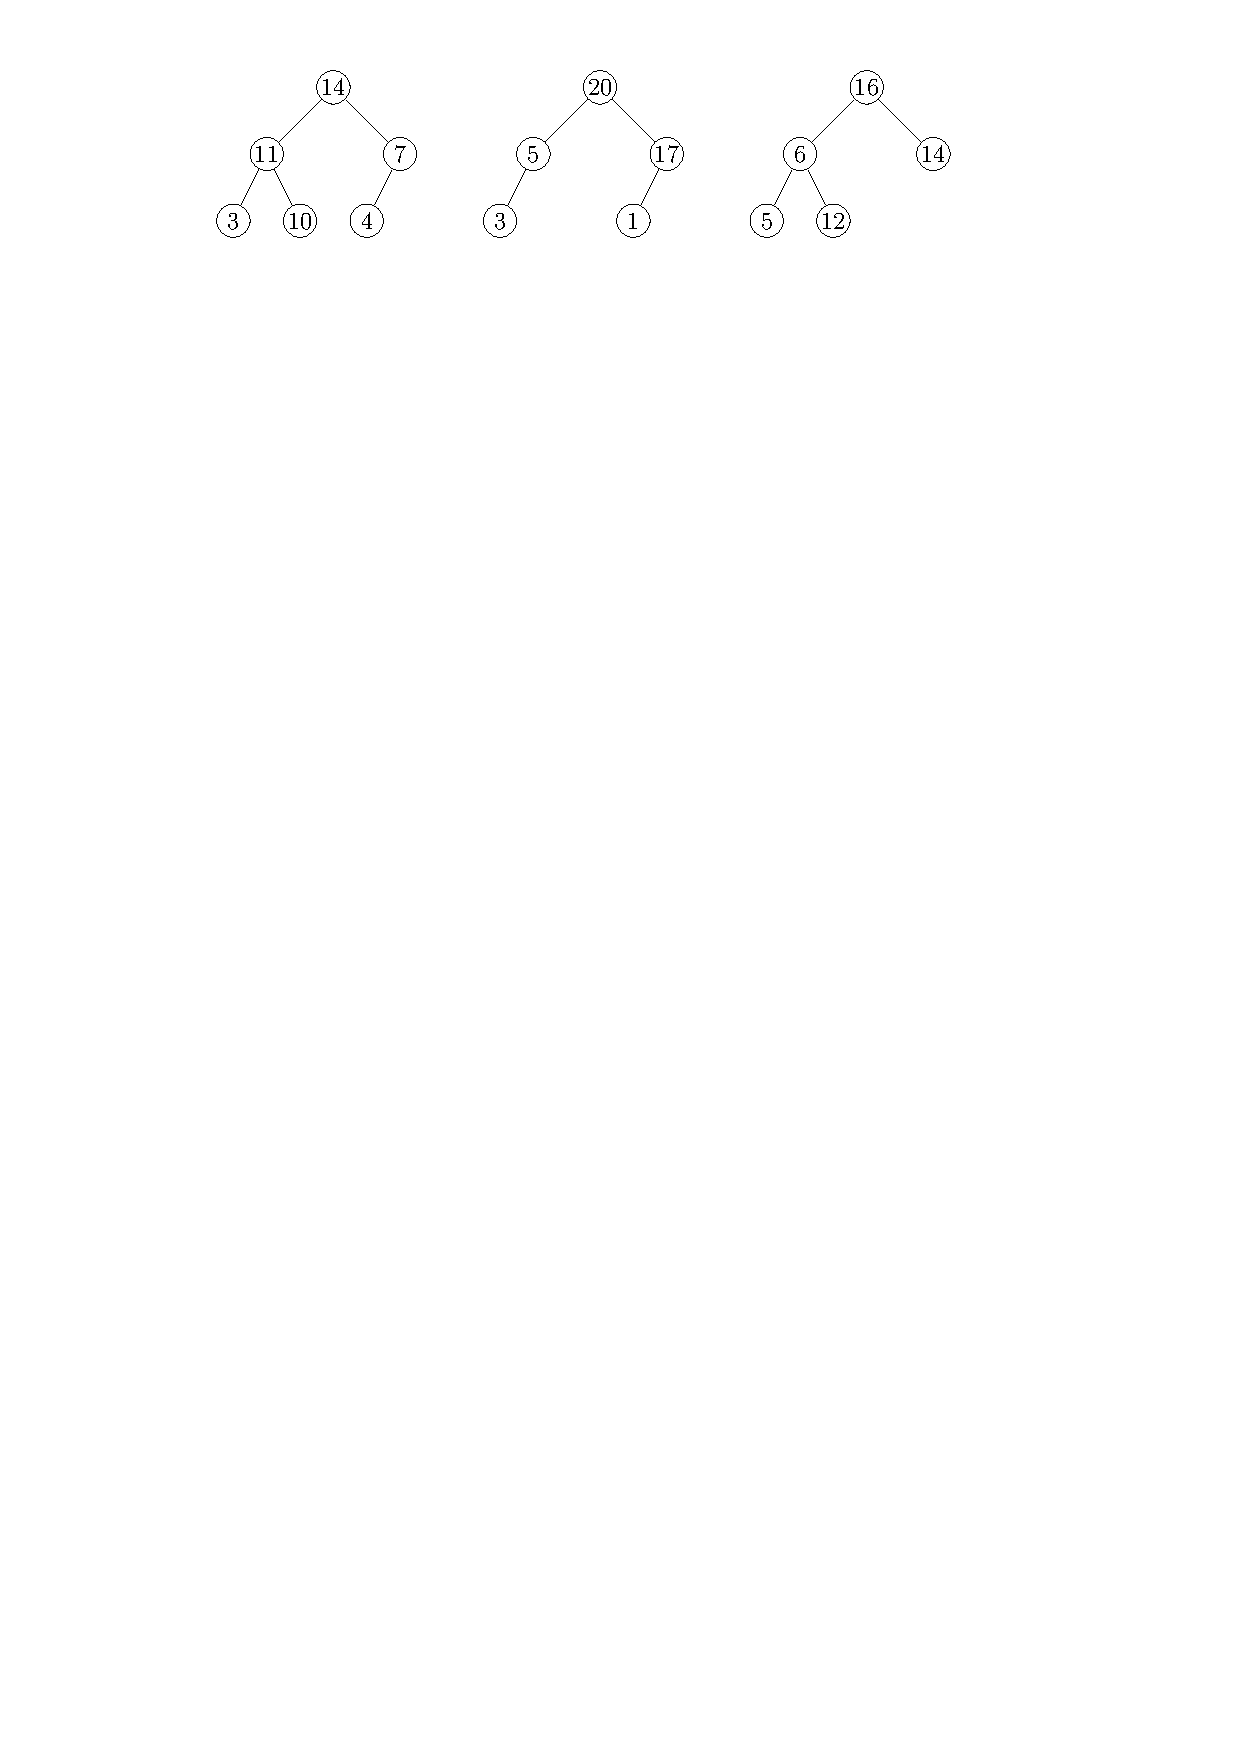
\includegraphics{heapsEx}
\end{center}
\end{Boxample}

A heap can implement a priority queue as follows. 
\begin{itemize}
\item Keys are stored in nodes. 
\item To insert a node, create a new leaf at the bottom level as far left as 
possible. Swap it upward until no swap is required. 
\item To delete the maximum, remove the root. Put the rightmost leaf in the root
 position. Swap it downward (choosing the larger child each time) until no swap 
is required. 
\end{itemize}

\begin{Boxample}
Example of heap insertion and deletion. 
\begin{center}
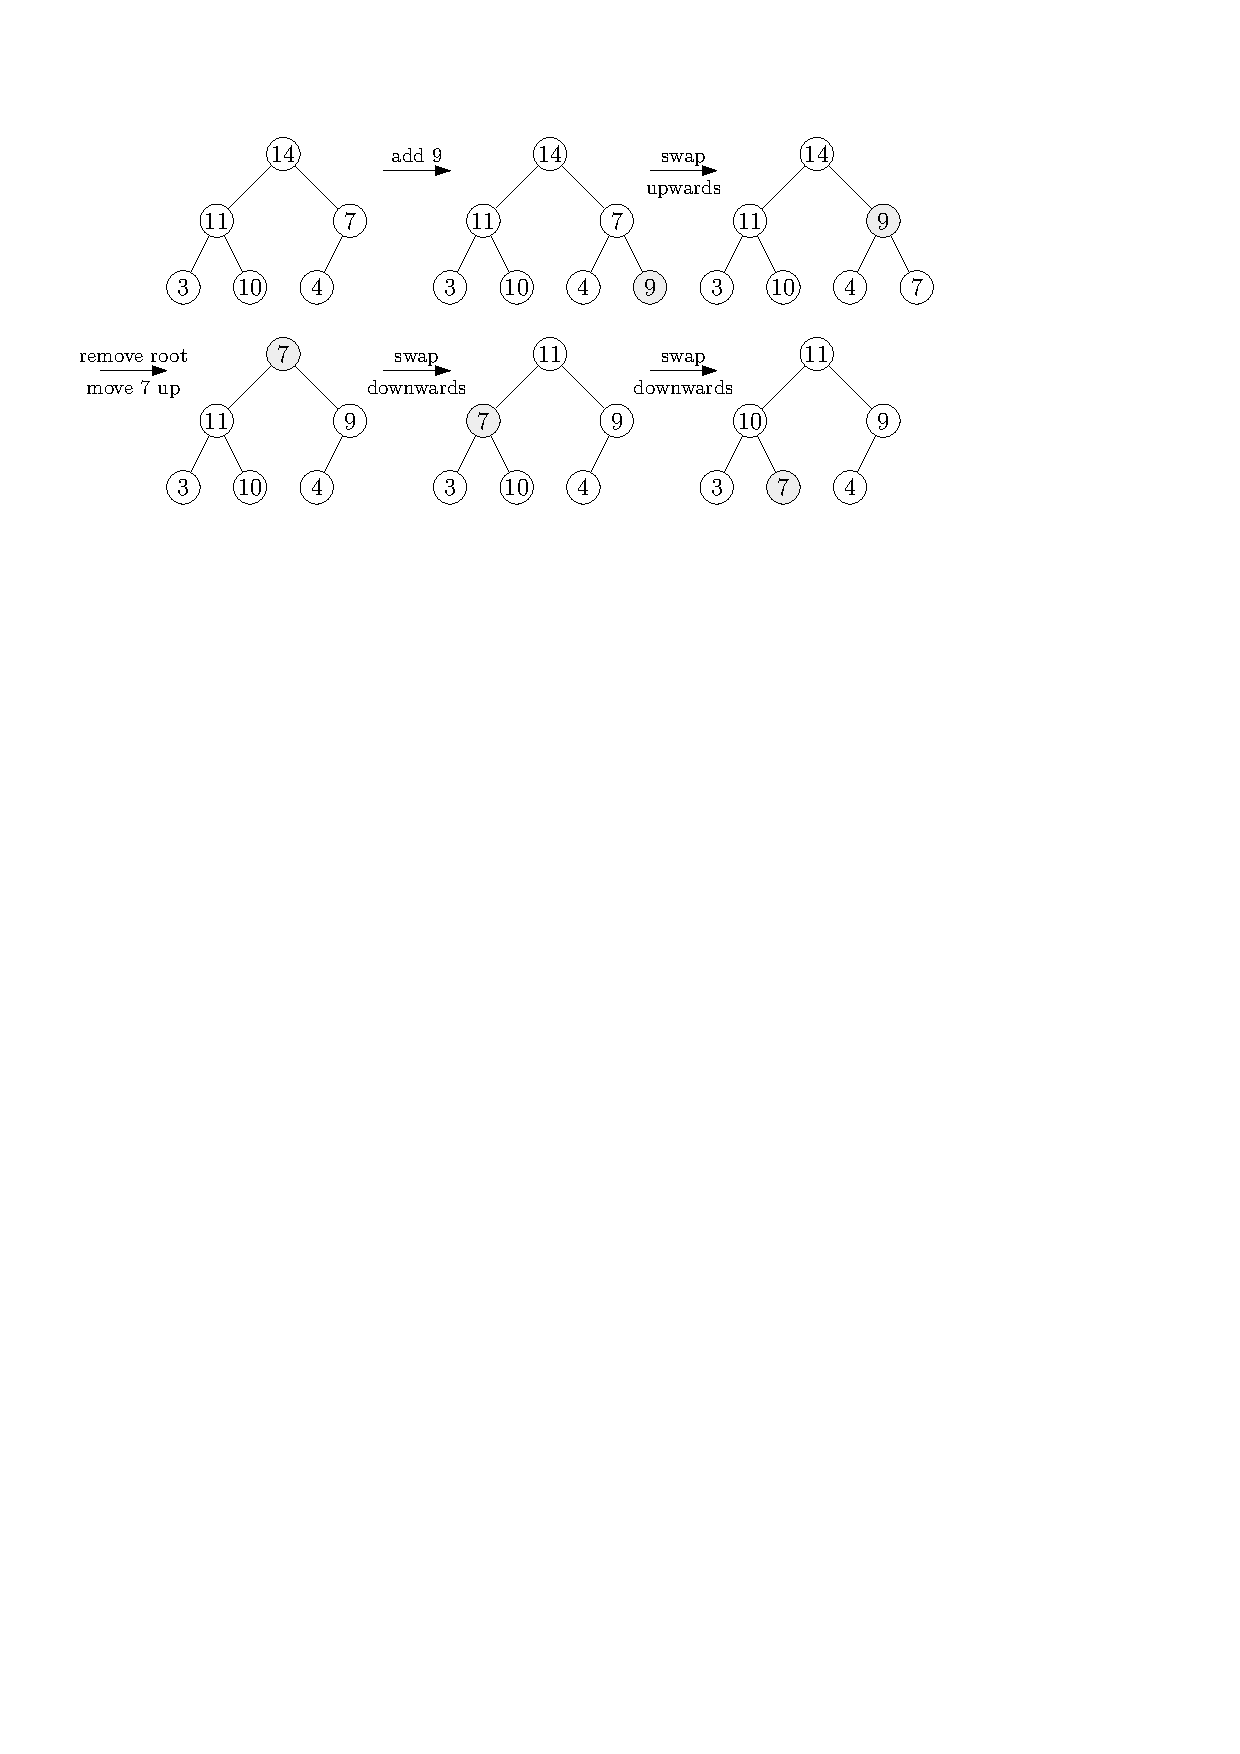
\includegraphics[width=1.0\textwidth]{heapInsertDelete}
\end{center}
\end{Boxample}

\section{Heapsort analysis}
\begin{itemize}
\item Building a heap using $n$ successive insertions takes time in 
$O(n\log n)$ since the tree has height in $O(\log n)$.
\item Deleting the root $n$ times, restoring the heap property each time, takes
 time in $O(n \log n)$.
\item Thus heapsort is a worst-case $\Theta(n \log n)$ sorting algorithm, like 
mergesort. 
%\item Detailed average-case analysis is more difficult, but the best and worst 
%case are not very different. Heapsort is not very sensitive to the input.
\end{itemize}

\section{How can we improve the algorithm?}
It turns out we can make heapsort work in-place without building a separate heap, 
because the tree structure is so restricted.

\section{Array representation of binary heap}
\begin{itemize}
  \item A binary heap can be represented \boldfont{implicitly} (without pointers) in an array. 
  \begin{itemize}
	\item Each node corresponds to an array index (starting with $1$). 
	\item The children of the node corresponding to index $k$ are in positions $2k$ (left) 
	and $2k+1$ (right). The keys are stored directly in the array.
  \end{itemize}
  \item To insert a key $x$, put it in position $n+1$ and swap as above.
  \item To delete the root, swap $a[1]$ with $a[n]$, and swap as above. 
  Note that deleted elements end up at the end of the array.
\end{itemize}

\begin{Boxample}[0]
Give the array representation of the binary heap.
\begin{center}
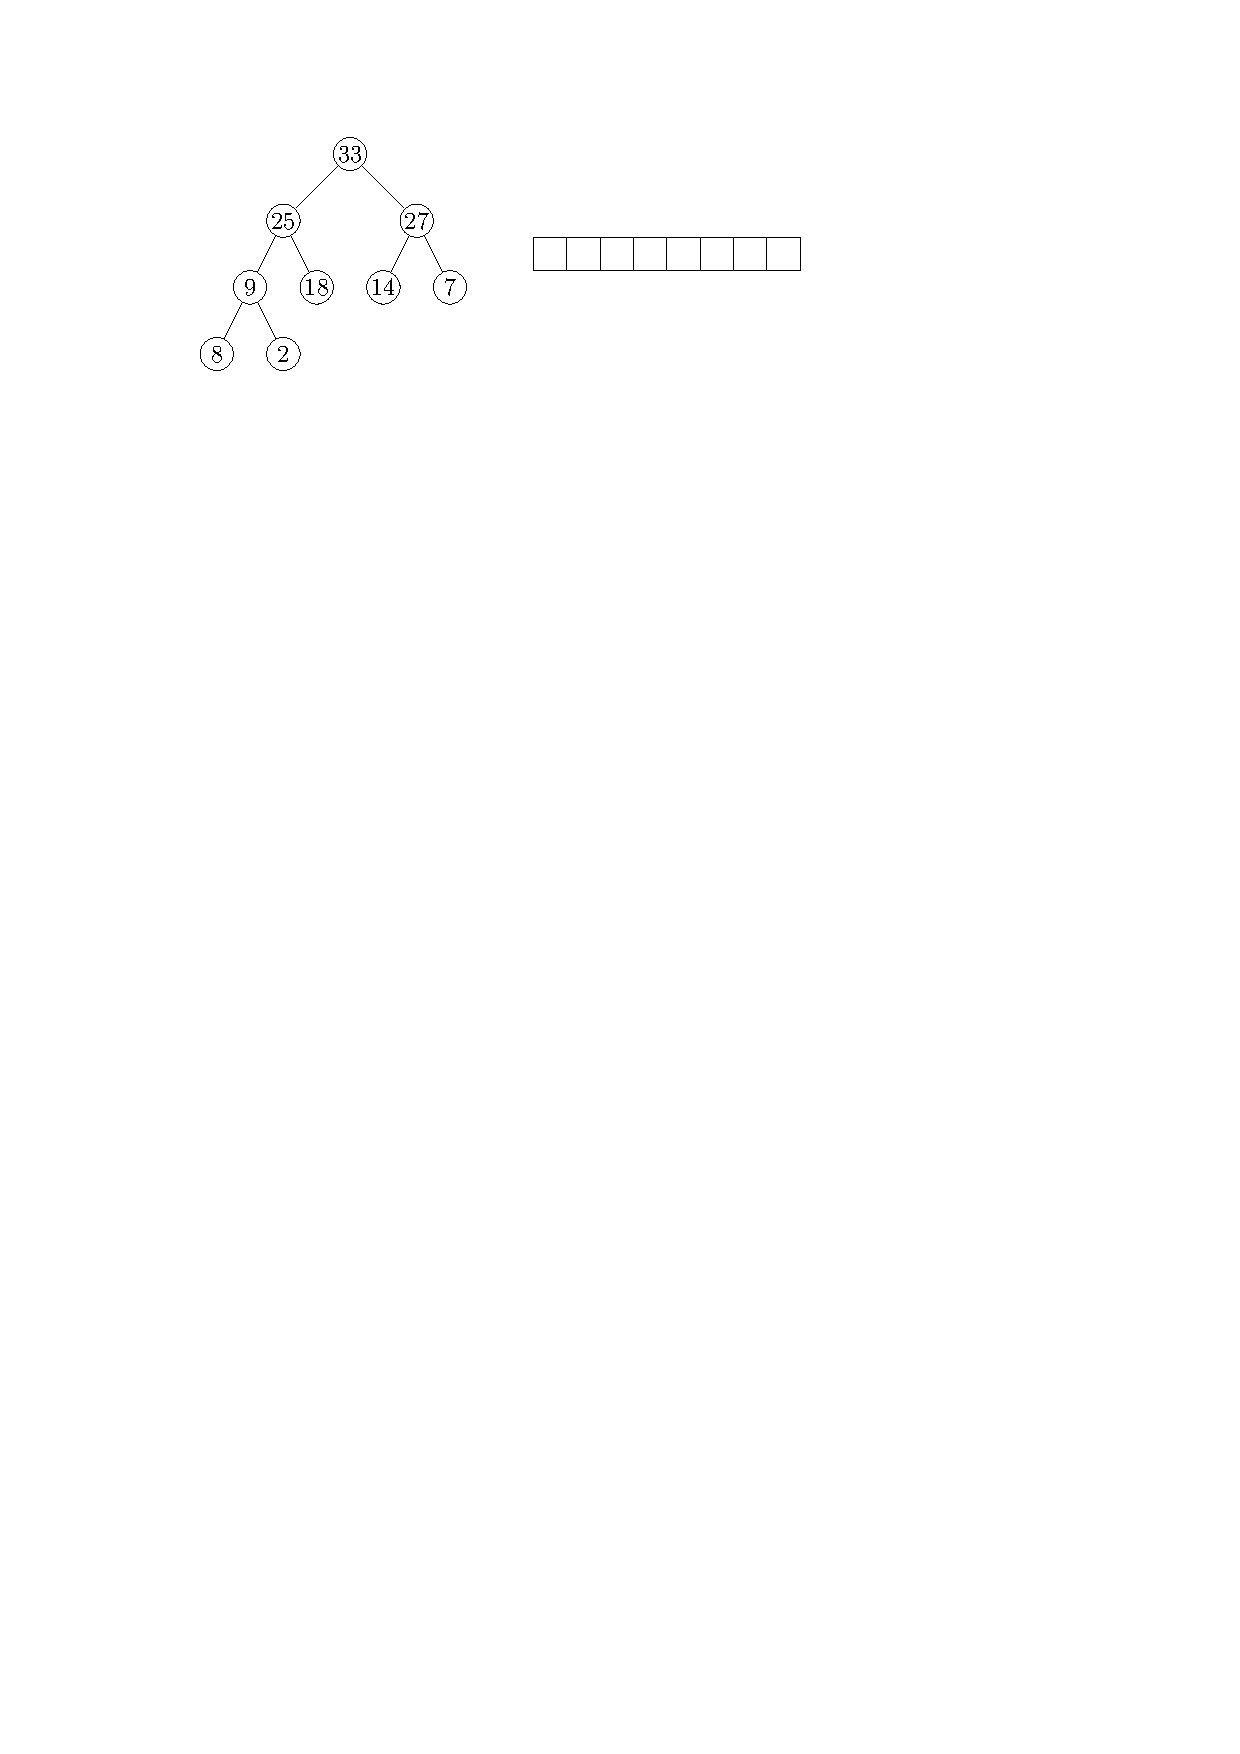
\includegraphics{heapArray}
\end{center}
\end{Boxample}

Note that for heapsort we only need the heap property at the end, but our method keeps it after inserting every element. 
Can we be more efficient? Yes - one way is to build a complete binary tree without the heap property, then
recursively heapify the left and right subtrees, and then let the root swap 
down to the right position. The recursion $T(n) = 2T(n/2) + \lg n$ describes the running time of the 
latter method: solution is $\Theta(n)$ (exact formula is tricky to guess).
 
This method can be rewritten to avoid recursion (``bottom-up") and to work 
in place in the array implementation. 

There is still serious research being done on better priority queue implementations.

\begin{Boxample}\label{ex:heapbuild}
Heap-building algorithm as in the first while-loop of \cref{alg:heapsort}.
\begin{center}
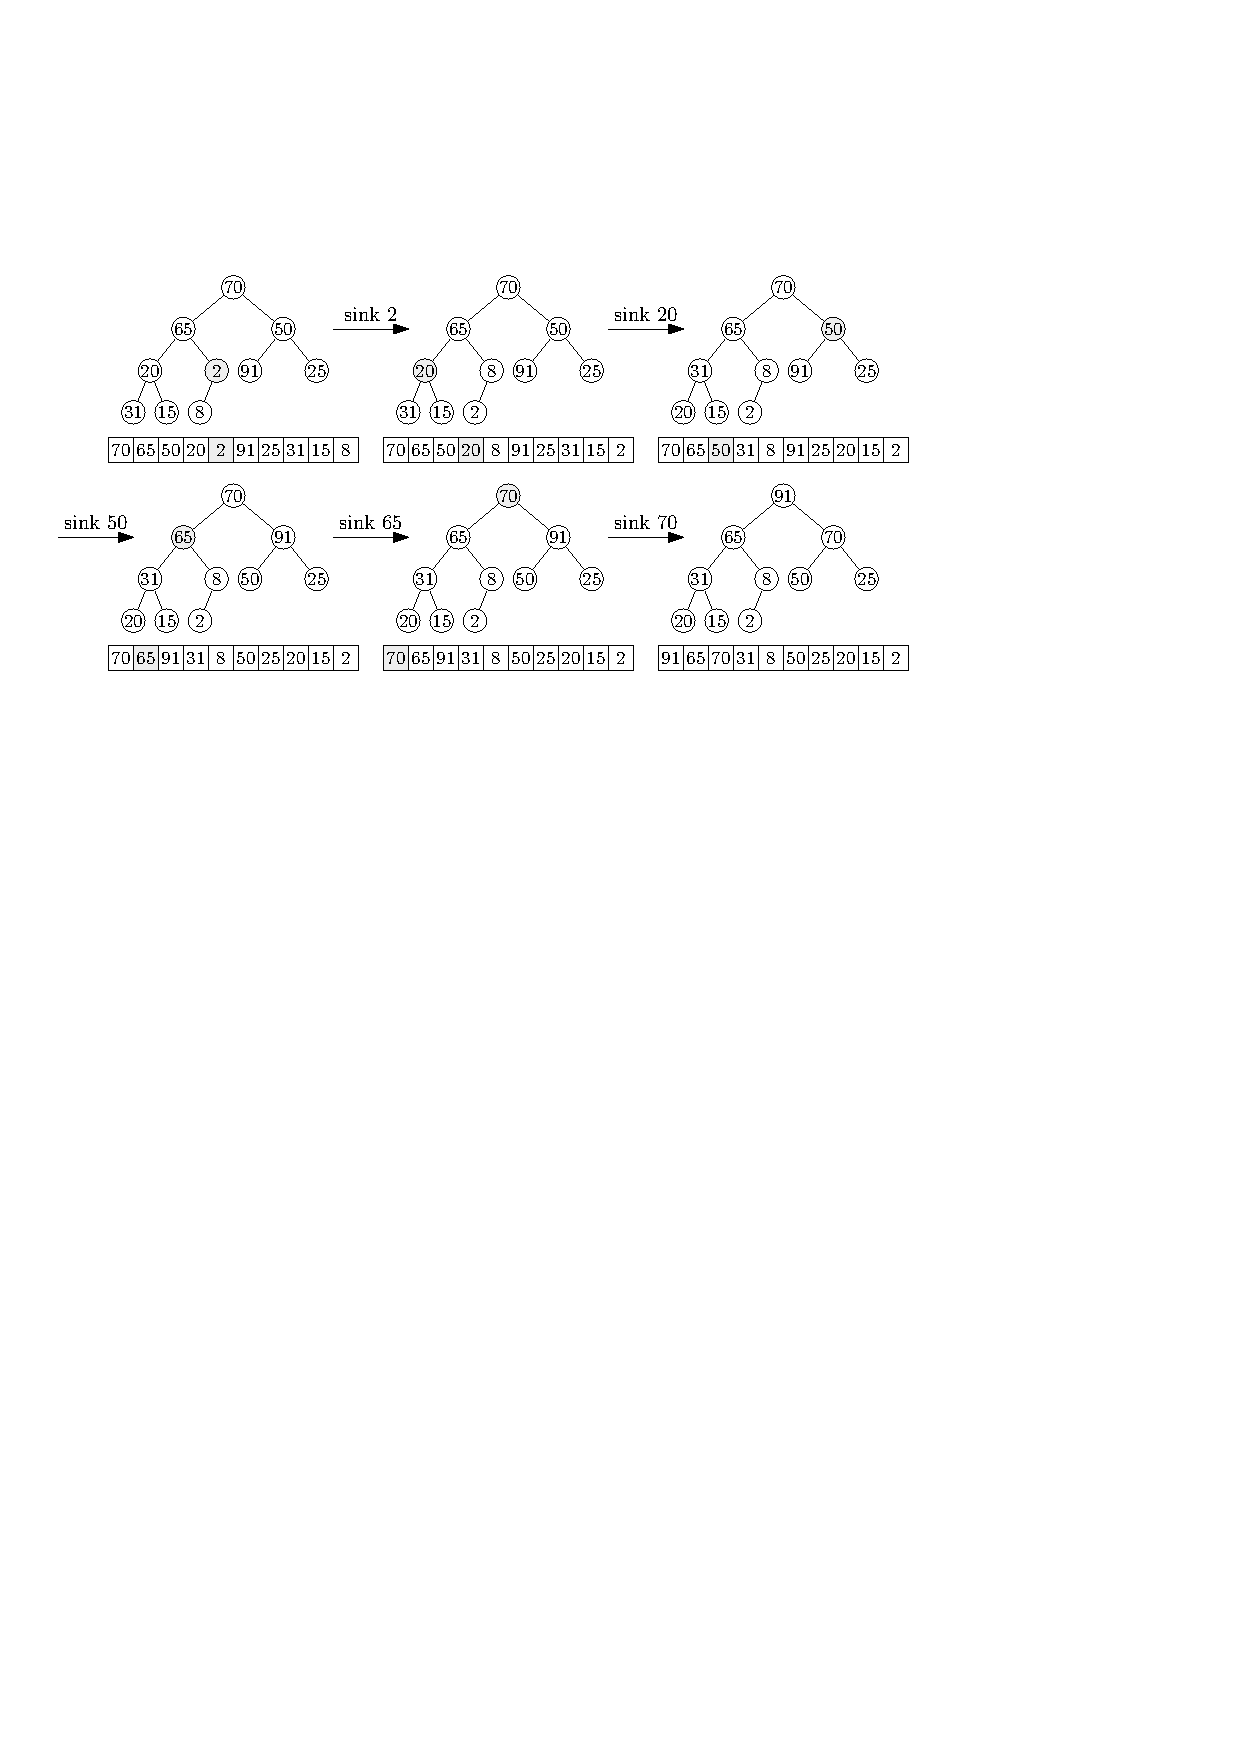
\includegraphics[width=1.0\textwidth]{heapBuild}
\end{center}
\end{Boxample}

\begin{algorithm}[H]
  \caption{Heapsort.}
  \label{alg:heapsort}
\begin{algorithmic}[1]
\Function{Heapsort}{array $a[0..n-1]$}
\State $k \gets n-1$ \Comment{index of last leaf in heap}
%\State $a\gets $ \texttt{heapify}($a$, $k$)
\State $i \gets \lfloor \frac{n-1}{2} \rfloor $
\While{$i\geq 0$} 
	\State \texttt{sink}$(a, i, k)$ \Comment{let element sink to its correct place}
	\State $i\gets i - 1$
\EndWhile \Comment{heap now built}
\While{$k > 0$}
	\State \texttt{swap}$(a[k], a[0])$
	\State $k \gets k - 1$
	\State \texttt{sink}$(a, 0, k)$ \Comment{let element at root sink to its correct place}
\EndWhile
\State \Return{$a$}\Comment{array is now sorted}
\EndFunction  
\end{algorithmic}
\end{algorithm}

\begin{Boxample}[0] Complete the last steps of Heapsort.
\begin{center}
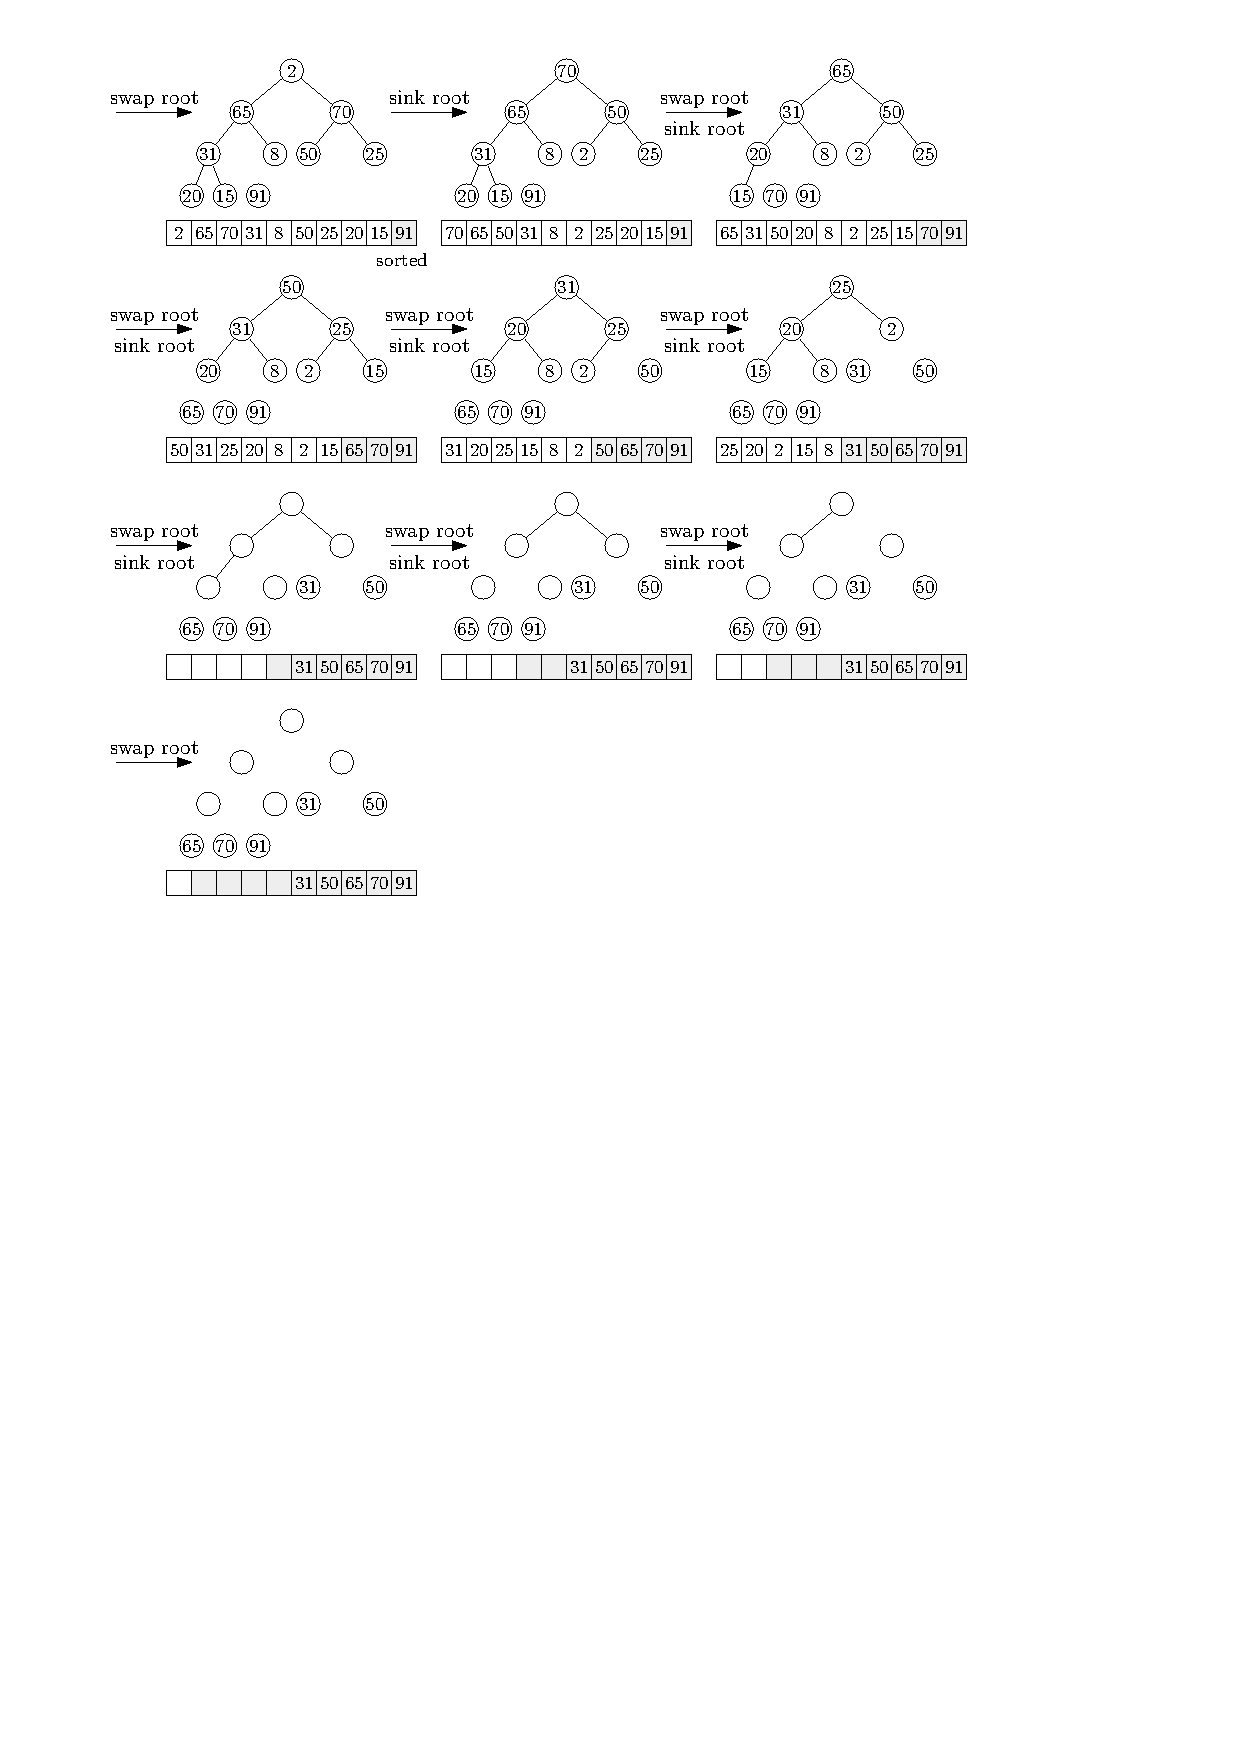
\includegraphics[width=1.0\textwidth]{heapSort}
\end{center}
\end{Boxample}

% There is still serious research being done on better priority queue implementations. %<< moved up for pagebreak


\chapter{Data selection and quickselect} %-------------------------------------------
\label{sec:qselect}

The table below gives a summary of results so far on sorting algorithms.
Running times give asymptotic order only. 
Shellsort analysis depends on the increments used, and is difficult. 
Quicksort needs a stack of size $\Theta(\log n)$ for the recursion. 
Selection sort is stable for linked lists. 
Mergesort is in-place for linked lists.

\begin{center}
\begin{tabular}{|c|c|c|c|c|c|} \hline 
Method & Worst & Average & Best & Stable? & In-place? \\
\hline
Insertion & $n^2$ & $n^2$ & $n$ & Yes & Yes \\
Selection & $n^2$ & $n^2$ & $n^2$ & No & Yes \\
Shellsort & ?? & ?? & $n$ & No & Yes \\
Mergesort & $n \log n$ & $n \log n$ & $n \log n$ & Yes & No \\
Quicksort & $n^2$ & $n \log n$ & $n \log n$ & No & Almost \\
Heapsort & $n \log n$ & $n \log n$ & $n \log n$ & No & Yes \\
\hline
\end{tabular}
\end{center}


\section{Selection}
We want to consider a related but different topic. Fix $r$ with $1\leq r \leq n$. 
We want to find the element with the $r$th key from an input list (the $r$th \defnfont{order statistic}). 
This should be easier than sorting! 

\begin{Boxample}[5]
Suppose that we build a priority queue and repeatedly extract elements until we get the one we want.
What is the asymptotic running time in terms of $n$ and $r$?

\end{Boxample}

\section{Quickselect}
One good approach is to use the quicksort idea. At each stage we only need to 
make a recursive call on one half of the array because we know where the pivot 
is relative to the desired element. This algorithm is called \defnfont{Quickselect}.

\begin{algorithm}[H]
  \caption{Quickselect.}
  \label{alg:quickselect}
\begin{algorithmic}[0]
\Require{$0 \leq i \leq j \leq n-1$, $1\leq r \leq j-i+1$}
\Function{quickselect}{list $a[0..n-1]$, int $i$, int $j$, int $r$}
	\If{$i \leq j$}
		\State $p \gets a[i]$ \Comment{pivot element}
		\State $q \gets \Call{partition}{a, i,j,p}$ \Comment{put $p$ in correct position}
		\If{$q-i=r-1$}
			\State \Return{$a[r-1]$}
		\ElsIf{$q-i > r-1$}
			\State $\Call{quickselect}{a,i,q-1,r}$ \Comment{look in left half}
		\Else{}
			\State $\Call{quickselect}{a,q+1,j,r-q+i-1}$ \Comment{right half}
		\EndIf
	\EndIf
%\State \Return{$a$}
\EndFunction  
\end{algorithmic}
\end{algorithm}

\begin{Boxample}[1]
Execute quickselect on the array below. Hint: You have to make one recursive call to the left and one to the right.
\begin{center}
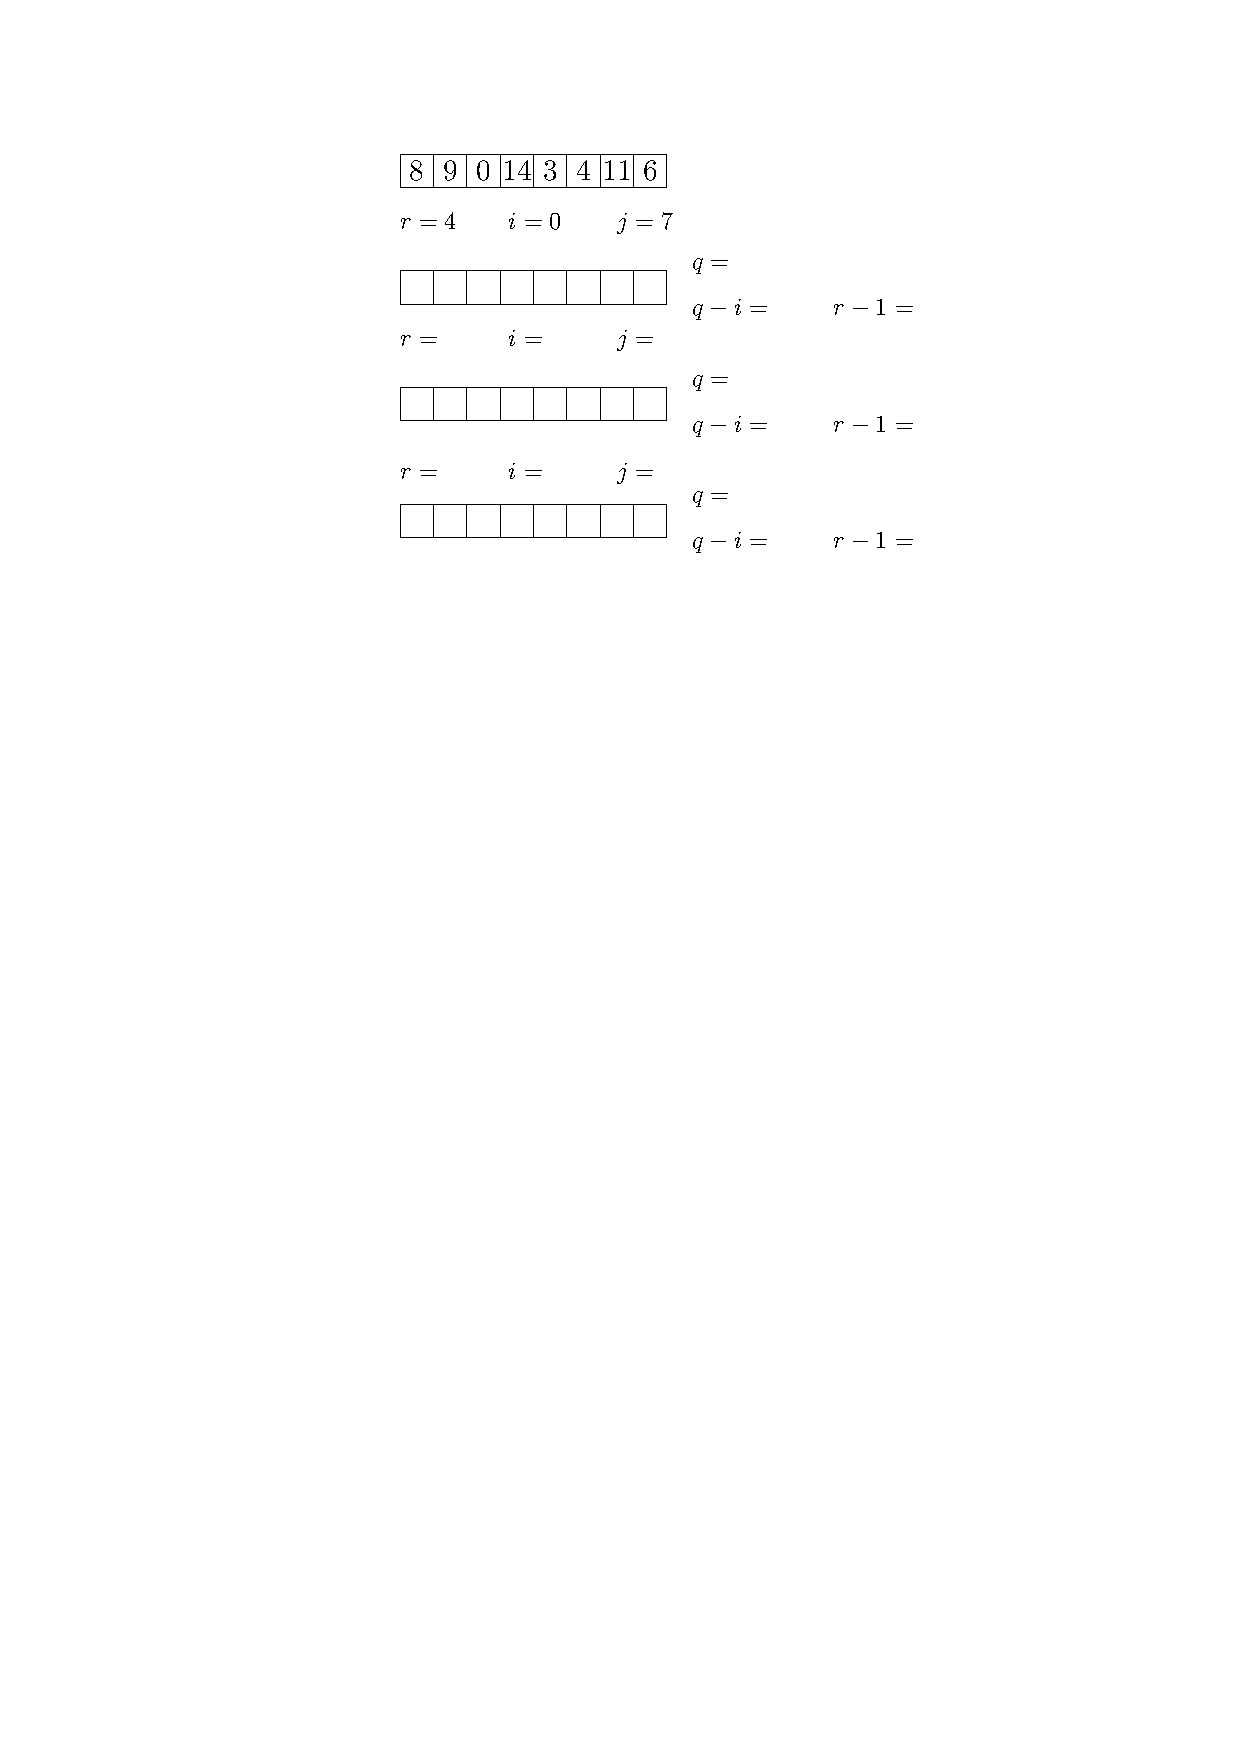
\includegraphics{QuickSelect} 
\end{center}
\end{Boxample}

% \paragraph{Questions}
% \begin{itemize}
% \item What is the average-case running time of quickselect?
% \item Is quickselect the best we can do?
% \end{itemize}

\section{Quickselect analysis}
The recurrence for the average number of comparisons has the form 
$$E(n) = n + \frac{1}{n} \sum_{i=0}^{n-1} E(p)\text{.}$$

This has a solution that is $\Theta(n)$, via the same method used for the quicksort recurrence.

\begin{Boxample}[6]
Solve the quickselect recurrence above.
\end{Boxample}

The worst case running time is still quadratic, for the same reason as for quicksort.

\section{How can we improve quickselect?}
There is another divide-and-conquer algorithm (see Wikipedia, ``Median of medians") that is worst-case linear, 
but much more complicated and never used in practice. 
Note that if it did work well in practice, we would use it to find an optimal (i.e. median) pivot, 
and thereby achieve $O(n\log n)$ worst case running time for quicksort.


